\documentclass[dvipdfmx,8pt]{beamer}

\usepackage[T1]{fontenc}
\usepackage[ansinew]{inputenc}

\usepackage{bxdpx-beamer} % dvipdfmxなので必要
\usepackage{pxjahyper} % 日本語のしおり用
% \usepackage{minijs} % フォントの設定?pLaTeX, upLaTaXなら不要

\usepackage{url} % 文中にリンク張る用
\usepackage{comment} % 複数行コメントアウト用
\usepackage{amsmath} %数式用
\renewcommand{\kanjifamilydefault}{\gtdefault} % 既定をゴシック体に変更

\newcommand{\probability}[1]{\mathrm{Pr}[{#1}]}

% \usetheme{metropolis}
\AtBeginSection{\frame{\sectionpage}} % Section毎に見出しを追加

\title{The Elements of Statistical Learning\\Chap.18: High-Dimensional Problems: $p \gg N$}
\date{\today}
\author{Kosuke Kito}

\begin{document}
  \maketitle
  \section{Introduction\\p.653-}
  \begin{frame}{本日のお題 - $p \gg N$ 問題}
    特徴量の数がサンプル数よりもずっと大きいとき($p \gg N$)に困っちゃう話.
    \begin{itemize}
      \item 困っちゃうポイントは, high variance と overfitting
      \item simple, highly regularized な手法が使われる.
      \item 主な話題は以下の2つ.
      \begin{itemize}
        \item prediction
        \item feature selection, assesment
      \end{itemize}
    \end{itemize}
    \begin{figure}[htb]
      \centering
      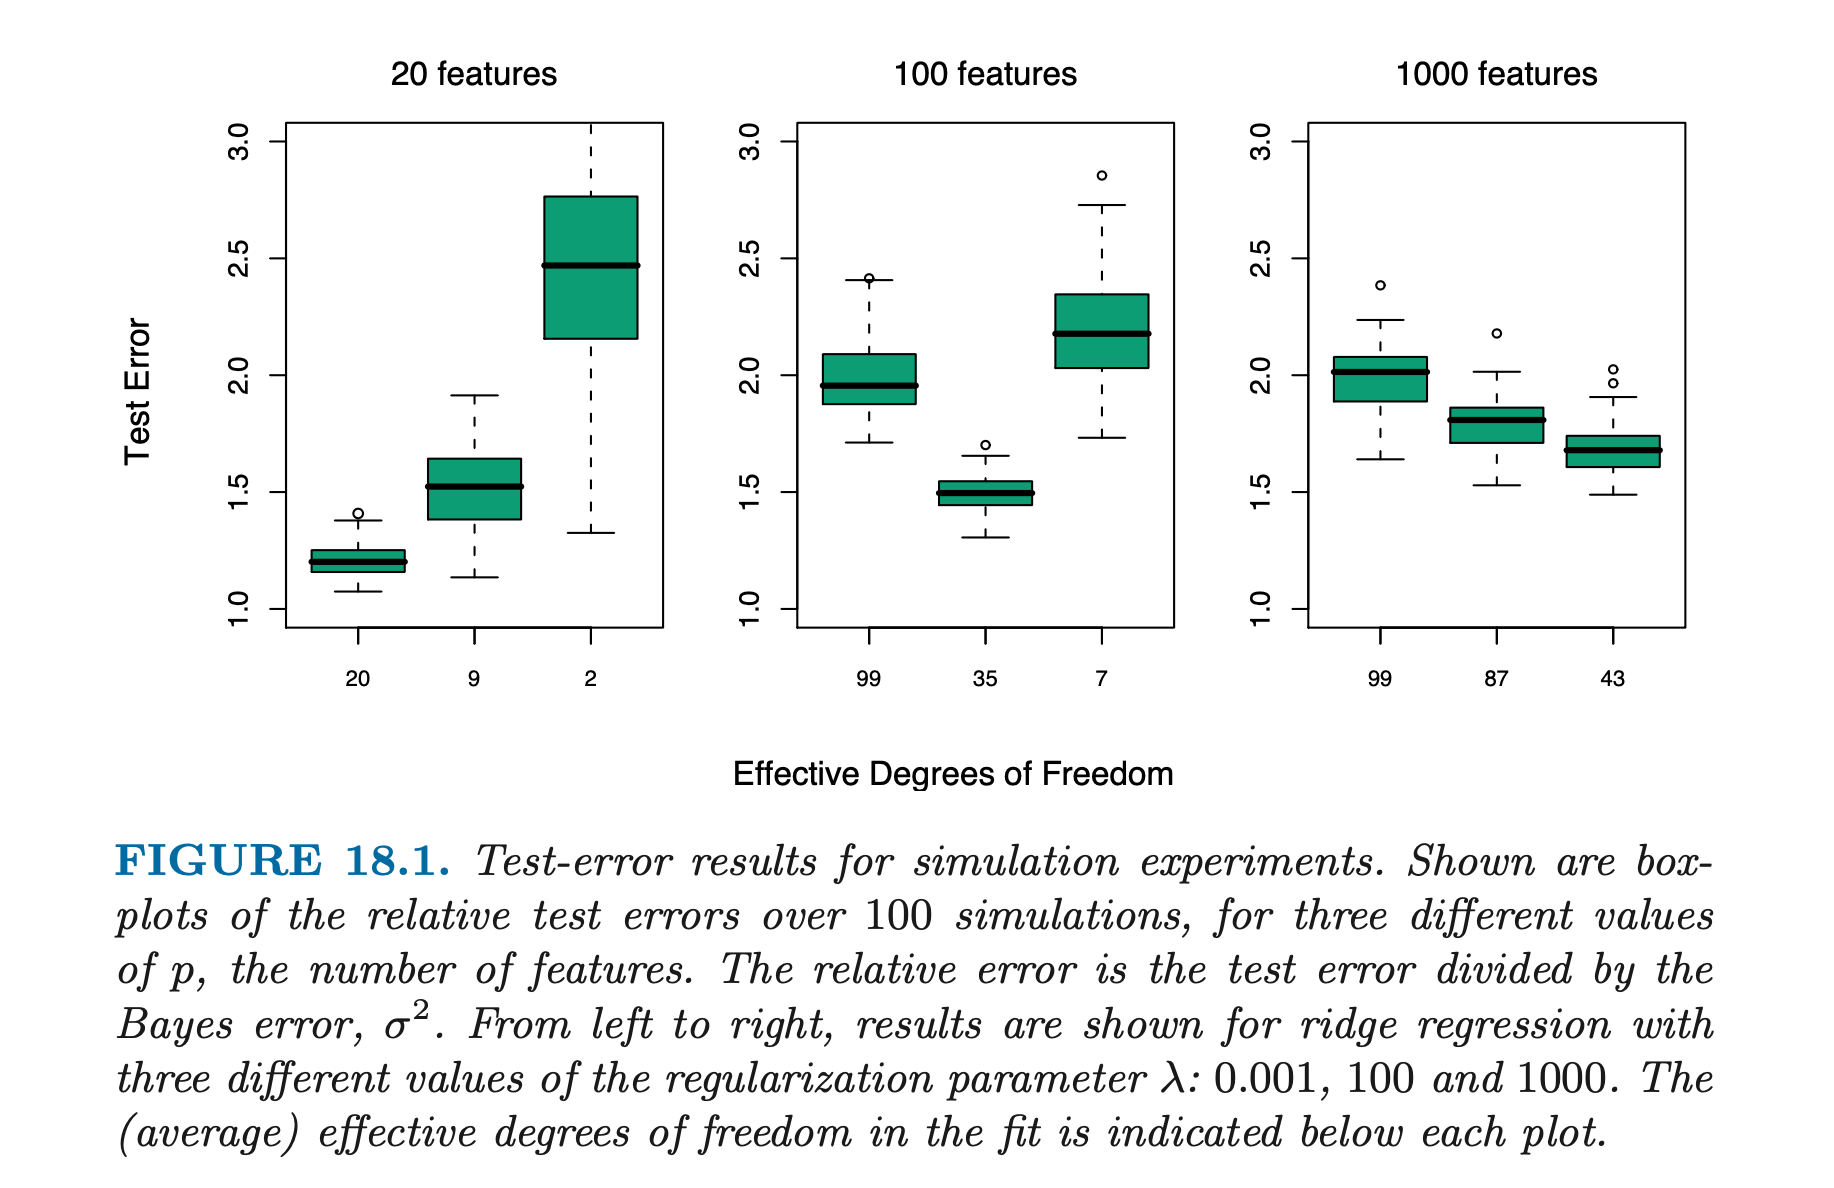
\includegraphics[width=5cm]{./images/test-error-in-high-demension.png}
    \end{figure}
  \end{frame}
  \begin{frame}{流れ}
    \begin{itemize}
      \item 流れを書く.
    \end{itemize}
  \end{frame}
  \section{LDAの正則化 - Diagonal LDA と NSC\\p.651-}
  \begin{frame}{LDAの復習1 - コンセプト}
    $p\gg N$問題の最初の回避策は, ``Diagonal LDA''という線型判別法の強烈な正則化バージョン.

    とりあえず, LDAの復習. (不要であれば飛ばします. )
    \begin{itemize}
      \item 分類のための手法.
      \item 各入力$x$に対して, 事後確率$\probability{k \mid X=x}$が最大になるクラス$k$をクラスの推定値とする.
      \item 各クラス内で, 入力変数は多変量ガウス分布に従うと仮定.
      \item 各クラスのクラス内分散が等しいと仮定. \\
        →クラス間の境界が線形になる.
      \item 数式で書くと次ページの流れ.
    \end{itemize}
  \end{frame}
  \begin{frame}{LDAの復習2 - 定式化と計算}
    \begin{itemize}
      \item 各クラス内の分布はガウス分布と仮定.
        \[
          \probability{X=x | G=k}=\frac{1}{(2 \pi)^{\frac{p}{2}}|\Sigma|^{\frac{1}{2}}}e^{-\frac{1}{2}(x-\mu_k)^\mathrm{T}\Sigma(x-\mu_k)}
        \]
      \item ベイズの定理より事後確率は以下.
        \[
          \probability{k \mid X=x}=\frac{\probability{X=x | G=k}\probability{G=k}}{\sum_l\probability{X=x | G=l}\probability{G=l}}
        \]
      \item 事後確率の大小比較のため対数比(log-ratio)を見る.
        \begin{eqnarray*}
          \log \frac{\probability{k \mid X=x}}{\probability{l \mid X=x}} &=& \log \frac{\pi_k}{\pi_l}-\frac{1}{2}(\mu_k+\mu_l)^{\mathrm{T}}\Sigma^{-1}(\mu_k-\mu_l)+x^{\mathrm{T}}\Sigma^{-1}(\mu_k-\mu_l) \\
          &=& (\log\pi_k - \frac{1}{2}\mu_k^{\mathrm{T}}\Sigma^{-1}\mu_k+x^{\mathrm{T}}\Sigma^{-1}\mu_k)\\
          && - (\log\pi_l - \frac{1}{2}\mu_l^{\mathrm{T}}\Sigma^{-1}\mu_l+x^{\mathrm{T}}\Sigma^{-1}\mu_l)
        \end{eqnarray*}
      \item 結局, 点$x$がクラス$k$である度合い(discriminant score)は以下を評価すれば良い.
        \[
          \delta_k(x)=x^{\mathrm{T}}\Sigma^{-1}\mu_k-\frac{1}{2}\mu_k^{\mathrm{T}}\Sigma^{-1}\mu_k+\log\pi_k
        \]
    \end{itemize}
  \end{frame}
  \begin{frame}{Diagonal LDA - 線型判別法の強烈な正則化バージョン}
    \begin{itemize}
      \item 基本的なコンセプトは, 前述のLDAと同じ. 以下の条件を追加する.
        \[
          \Sigma = \mathrm{diag}(s_1, s_2, \dots , s_p) \quad \mbox{(対角行列)}
        \]
      \item すると, discriminant scoreは, (クラスに依らない定数$-x^\mathrm{T}\Sigma^{-1}x$を足して2倍することで, )以下になる.
        \[
          \delta_k(x)=-\sum_{j=1}^p\frac{(x_j-\bar{x}_{kj})^2}{s_j^2}+2\log\pi_k
        \]
      \item この discriminant score を使って, 以下のルールで分類する.
        \[
          C(x)=\mathrm{arg}\max_l\delta_l(x)
        \]
    \end{itemize}
  \end{frame}
  \begin{frame}{Diagonal LDA - 線型判別法の強烈な正則化バージョン}
    Diagonal LDAについて何点か補足.
    \begin{itemize}
      \item discriminant score は距離に見える.\\
        →Diagonal LDA は, 適当な標準化をしたデータにおける nearest centroid 法のようにも見える.
      \item 変数間の共分散が$0$という仮定を, 独立律(independent rule)ともいう.
      \item 高次元の時には, effective なことが多いらしい.
      \item この方法の欠点の一つは, 特徴量選択(feature selection)ができないこと. 高次元の入力の時には, 一部の変数を選び出せる方法を使いたい. \\
        →もっと正則化の条件を強めるとパフォーマンスがさらに上がるらしい.
      \item 次は, 特徴量選択が行われるような正則化の条件をかけたバージョンを考えます.
    \end{itemize}
  \end{frame}
  \begin{frame}{Nearest Shrunken Centroids}
    前出の Diagonal LDA = Nearest Centroid 法の centroid を縮小(shrinkage)させることで, 特徴量選択を行えるようにする.
    \begin{itemize}
      \item 基本的な計算は, Diagonal LDAと一緒.
      \item discriminant score の計算に使うcentroid を単純な平均$\bar{x}_{kj}$から変える.
      \item まず, あるパラメータ$X_j$のクラス$k$内での平均$\bar{x}_{kj}$と全体での平均$\bar{x}_j$の差を標準化する.
        \begin{columns}[t]
          \begin{column}{0.05\columnwidth}
            % 文頭を揃えるためのからのカラム
          \end{column}
          \begin{column}{0.6\columnwidth}
            \[
              d_{kj}=\frac{\bar{x}_{kj}-\bar{x}_j}{m_k(s_j+s_0b)}
            \]
            ただし, 各項は以下.
            \begin{align*}
              &m_k=\frac{1}{N_k}-\frac{1}{N}\colon \mbox{疑問点}\\
              &s_0=\mbox{小さな定数}\\
              &s_j\mbox{が小さい時に}d_{kj}\mbox{が大きくなりすぎないように}
            \end{align*}
            \begin{figure}
              \centering
              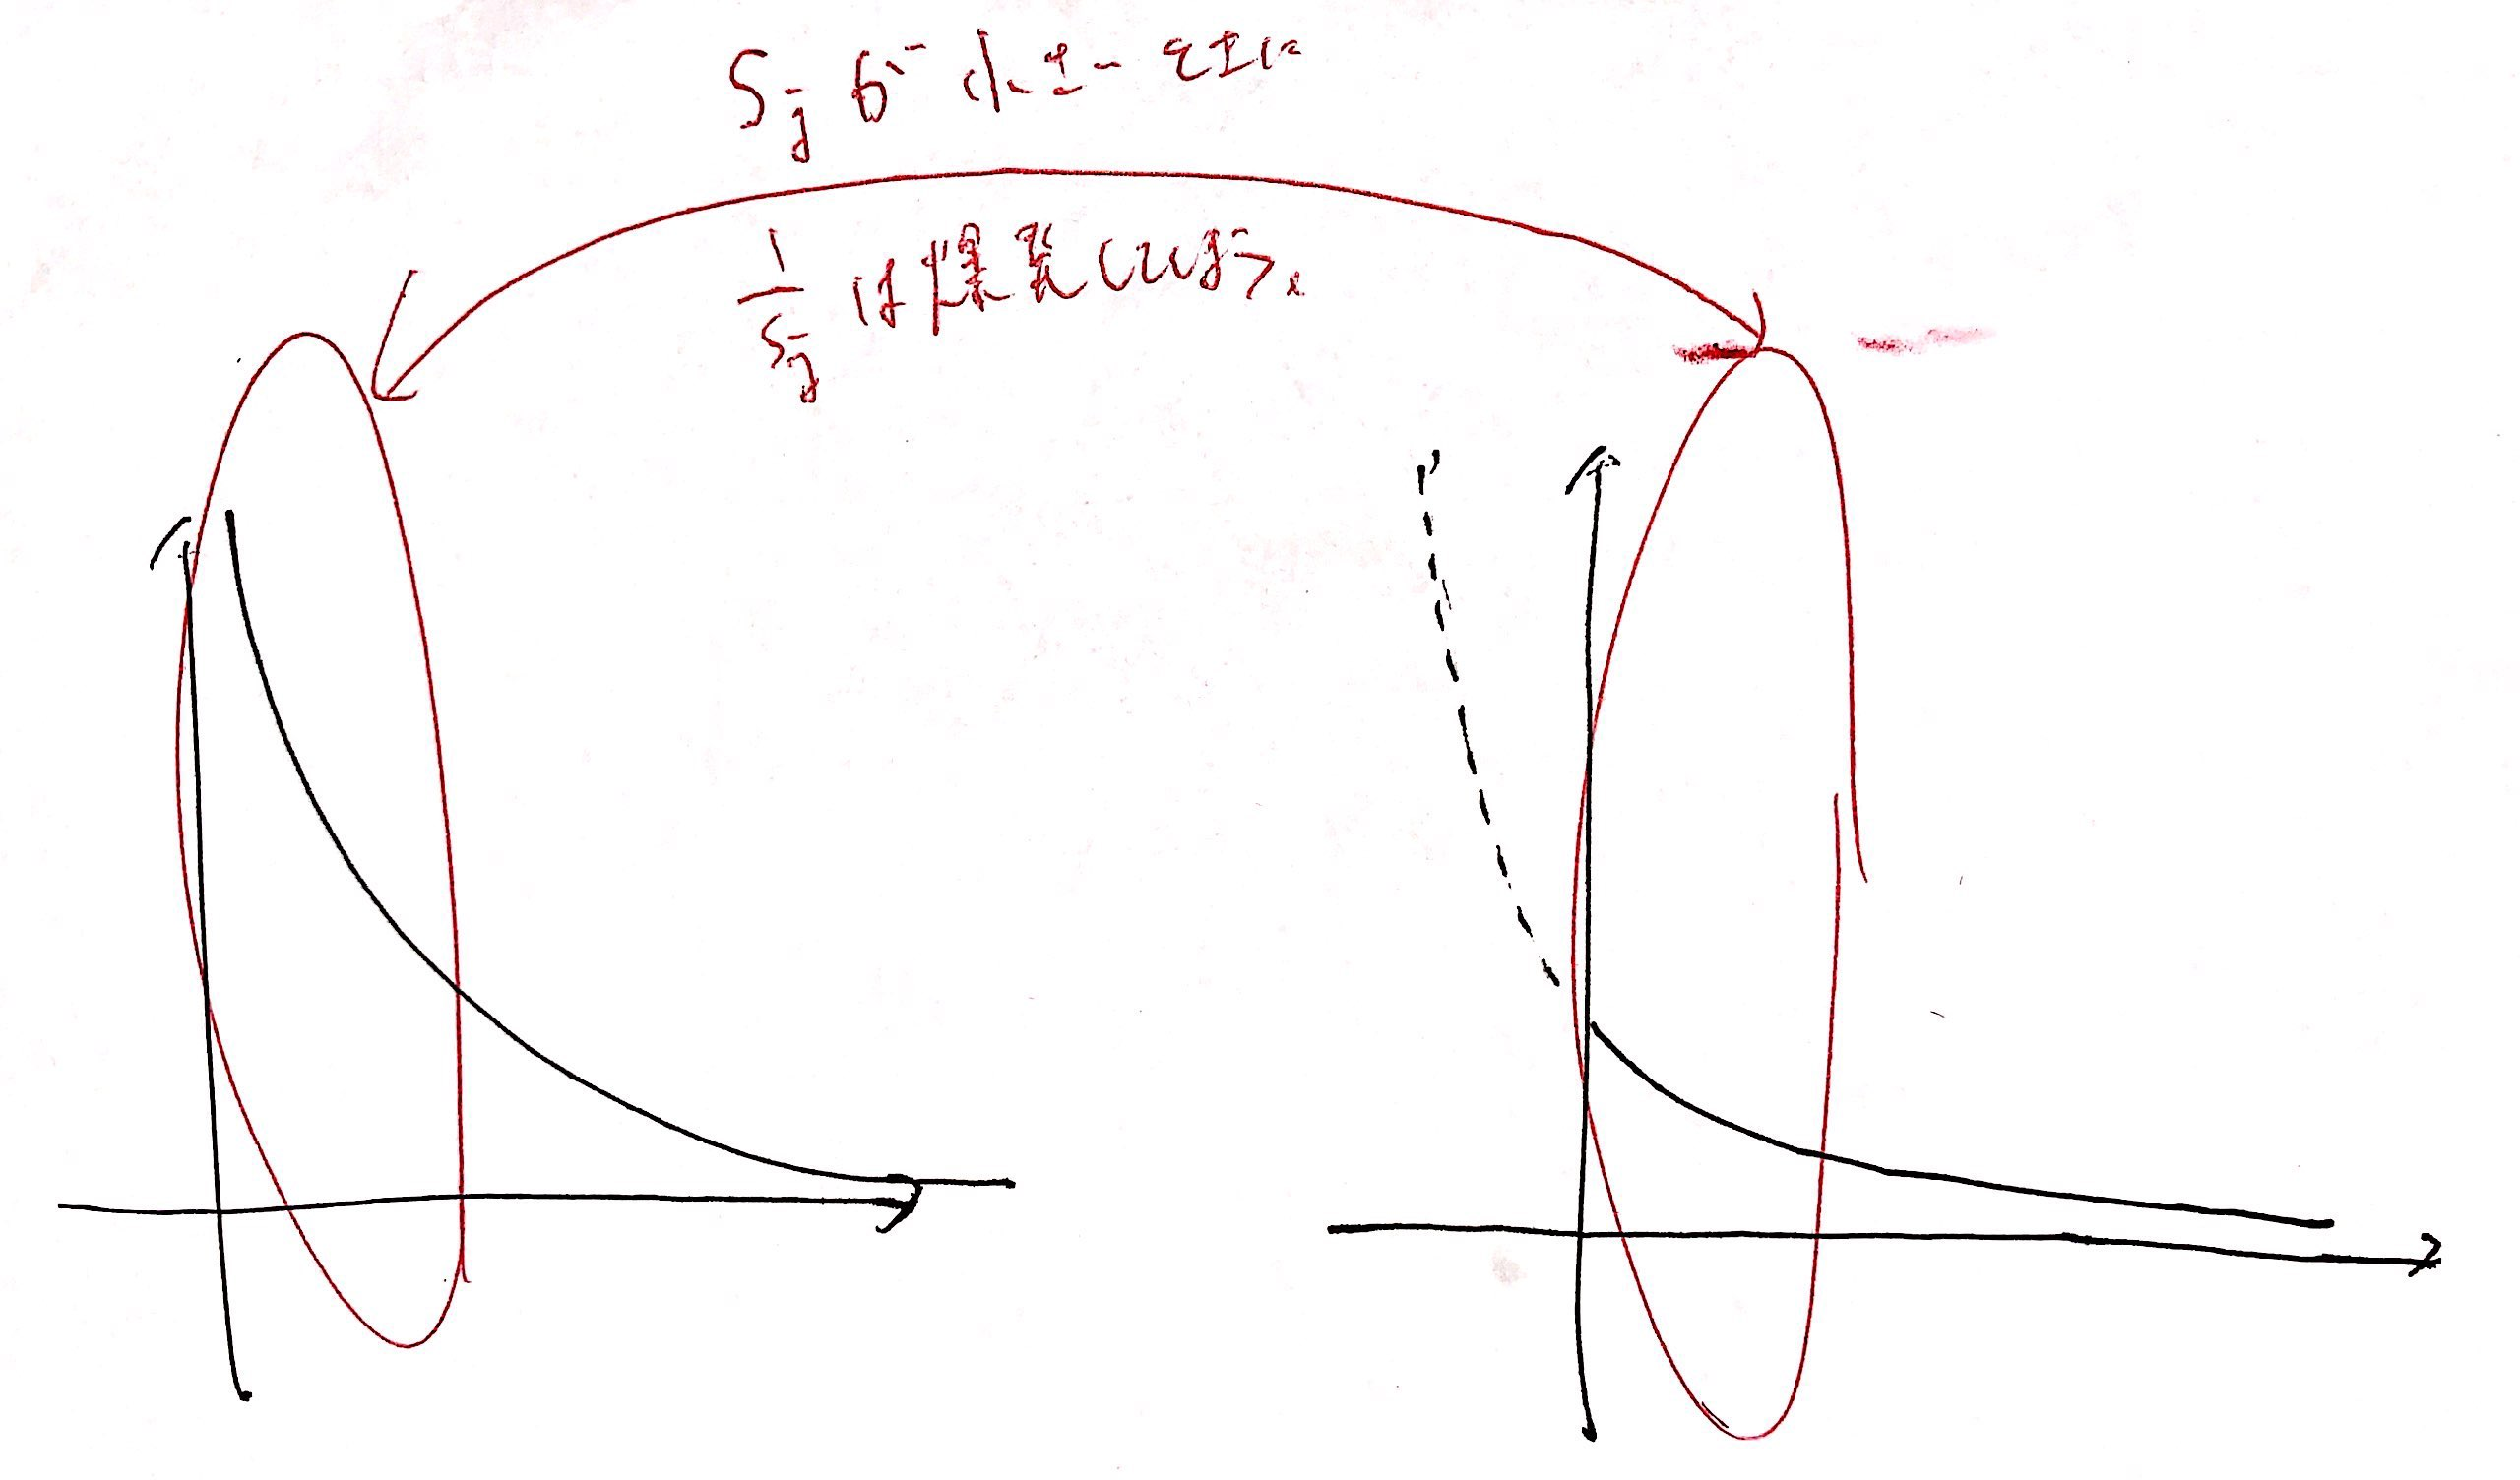
\includegraphics[width=3cm]{./images/nsc-normalization.jpg}
            \end{figure}
          \end{column}
          \begin{column}{0.35\columnwidth}
            \begin{figure}[htb]
              \centering
              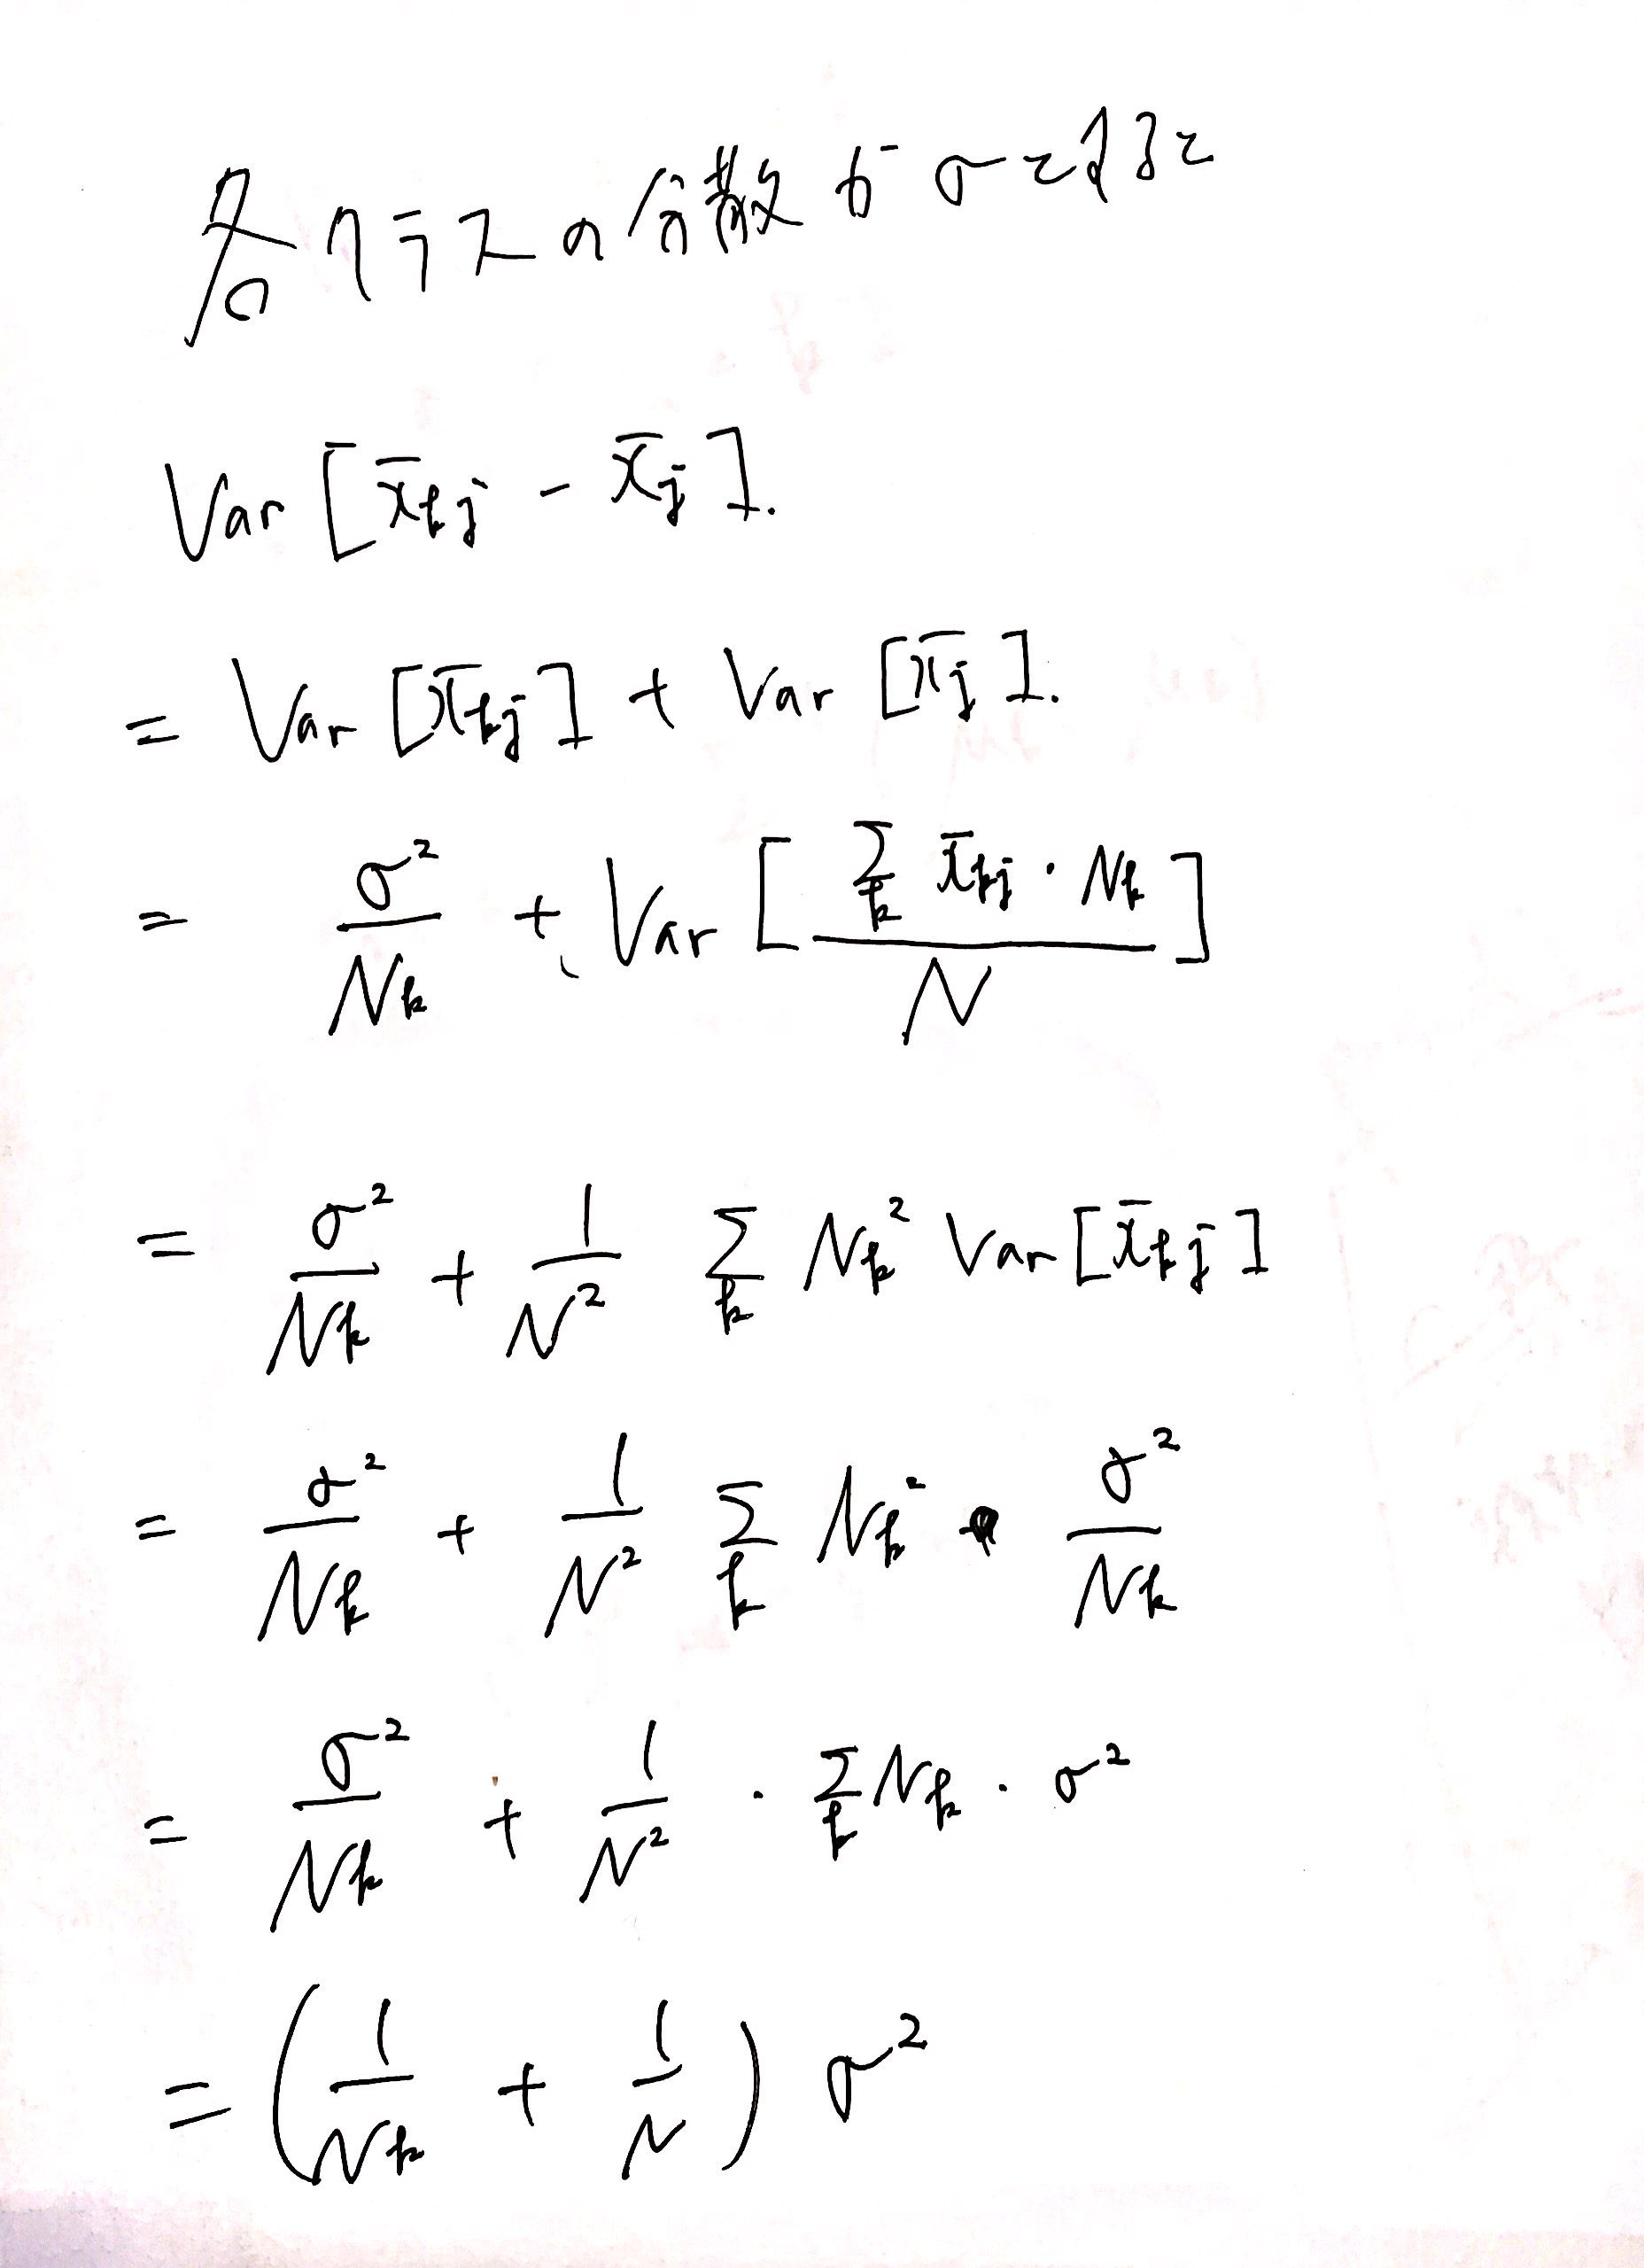
\includegraphics[width=3.5cm]{./images/nsc-variance-calc.jpg}
            \end{figure}
          \end{column}
        \end{columns}
    \end{itemize}
  \end{frame}
  \begin{frame}{Nearest Shrunken Centroids}
    \begin{itemize}
      \item この標準化された距離を soft-threshold
        \[
          d_{kj}'=\mathrm{sign}(d_{kj})(|d_{kj}|-\Delta)
        \]
        もしくは hard-threshold
        \[
          d_{kj}'=d_{kj}I(|d_{kj}|\ge\Delta)
        \]
        で縮小させる.
        \begin{figure}[htb]
          \centering
          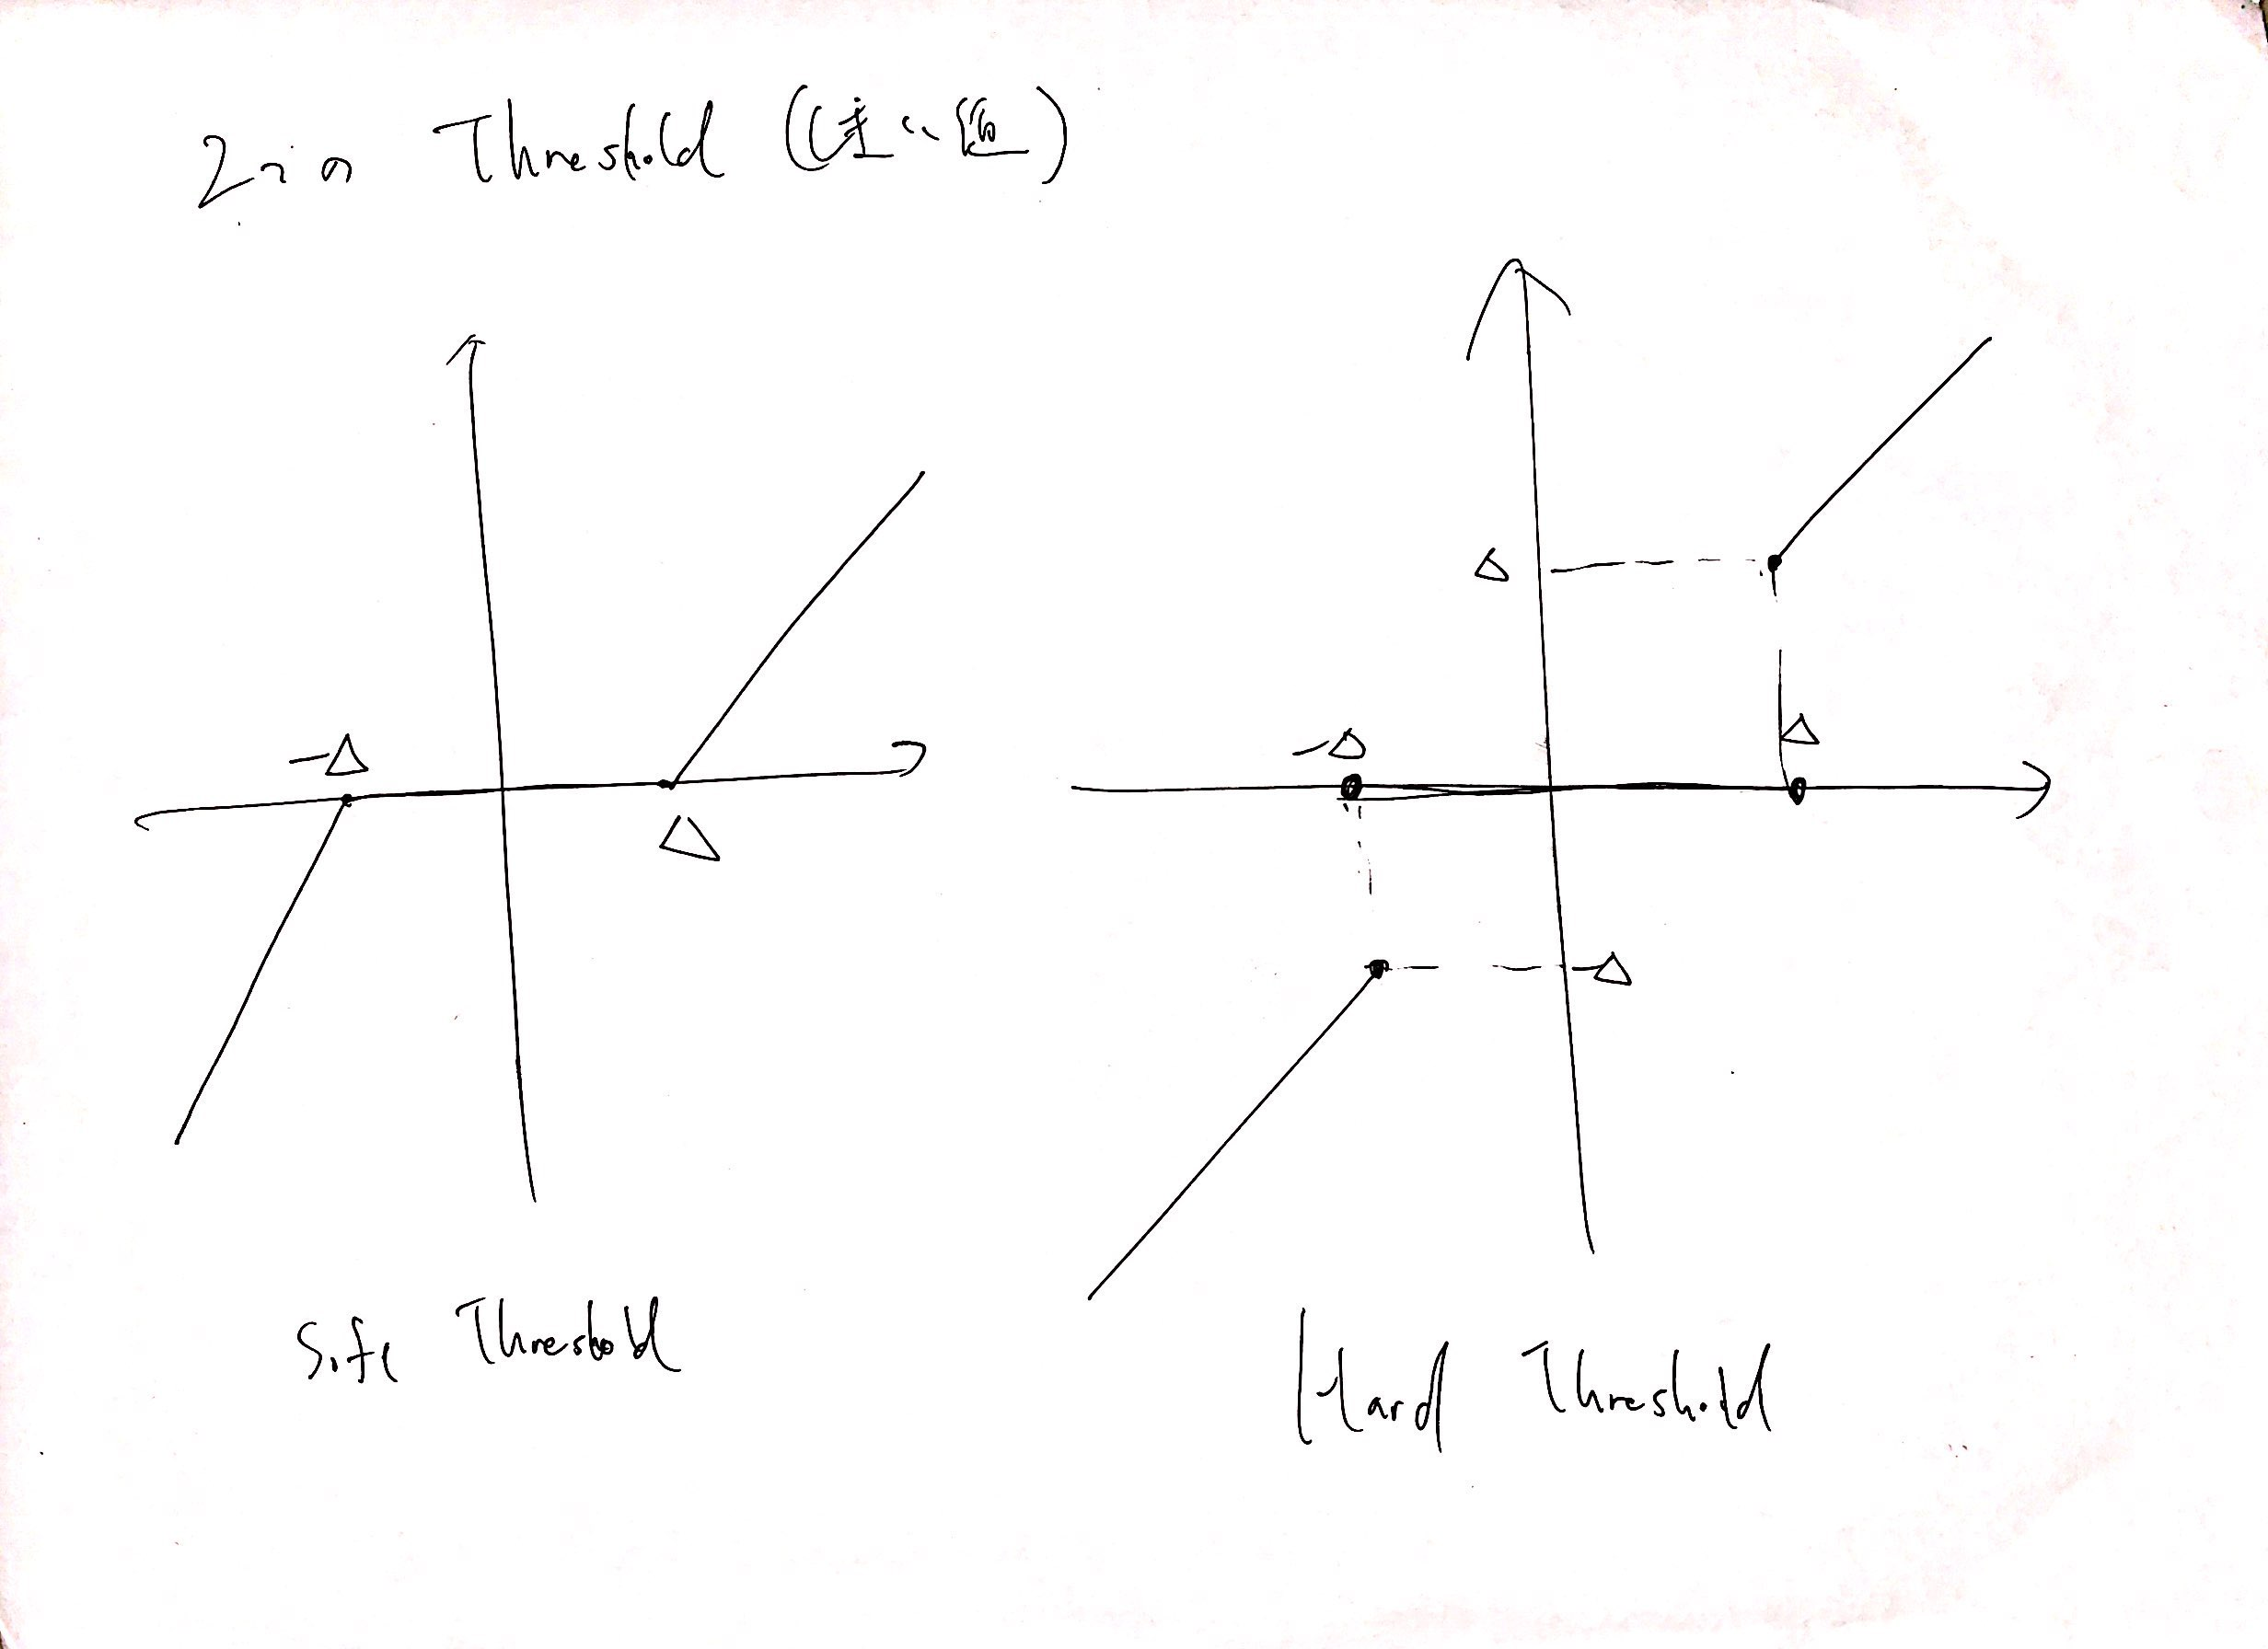
\includegraphics[width=4cm]{./images/thresholds.jpg}
        \end{figure}
      \item すなわち, 以下.
        \[
          \bar{x}_{kj}'=\bar{x}_j+m_k(s_j+s_0)d_{jk}'
        \]
        寄与の小さい特徴量を無視するようになっている.
      \item Diagonal LDA の discriminant score の$\bar{x}_{kj}$の代わりに, $\bar{x}_{kj}'$を使えば, NSCの完成.
    \end{itemize}
  \end{frame}
  \section{2次で正則化した線型分類\\p.654-}
  \begin{frame}{Regularized Discriminant Analysis}
    \begin{itemize}
      \item 判別分析の正則化を考える.
      \item 以前見た正則化は, LDA と QDA でバランスを取るために, 分散行列を以下で計算した.
        \[
          \hat{\Sigma}_k(\alpha)=\alpha\hat{\Sigma}_k+(1-\alpha)\hat{\Sigma}
        \]
      \item 今回は違うバージョン. 対角行列に近づけようとする.
        \[
          \hat{\Sigma}(\gamma)=\gamma\hat{\Sigma}+(1-\gamma)\mathrm{diag}(\hat{\Sigma})
        \]
      \item 上記の正則化で,  $\gamma=0$のときは, Diagonal LDA, すなわち, 縮小のない NSC と同じ.
      \item ridge回帰が分散共分散行列を対角行列に近づけようとするのと, 似ている.
        \[
          \hat{\beta}^{\mathrm{ridge}}=(\textbf{X}^{\mathrm{T}}\textbf{X}+\lambda\textbf{I})^{-1}\textbf{X}^{\mathrm{T}}\textbf{y}
        \]
      \item 線型判別を, 各クラスに数値を割り当てた線型回帰と思うと, ridge回帰との関連をより正確に記述できるそう.
    \end{itemize}
  \end{frame}
  \begin{frame}{ロジスティック回帰}
    \begin{itemize}
      \item 以下の式を使ってきた.
        \[
          \probability{G=k \mid X=x}=\frac{\exp(\beta_{k0}+x^{\mathrm{T}}\beta_k)}{\sum_l\exp(\beta_{l0}+x^{\mathrm{T}}\beta_l)}
        \]
      \item 対数尤度に正則化項を加えた以下を最大化する.
        \[
          \sum_{i=1}^N\log \probability{g_i\mid x_i}-\frac{\lambda}{2}\sum_{k=1}^K||\beta_k||^2
        \]
      \item 1個目の定式化だと, over-parametrized だけど, 正則化項のおかげでいい感じ.
      \item 定数項のみいい感じじゃないので, 適当に条件加えよう.
    \end{itemize}
    \begin{figure}[htb]
      \centering
      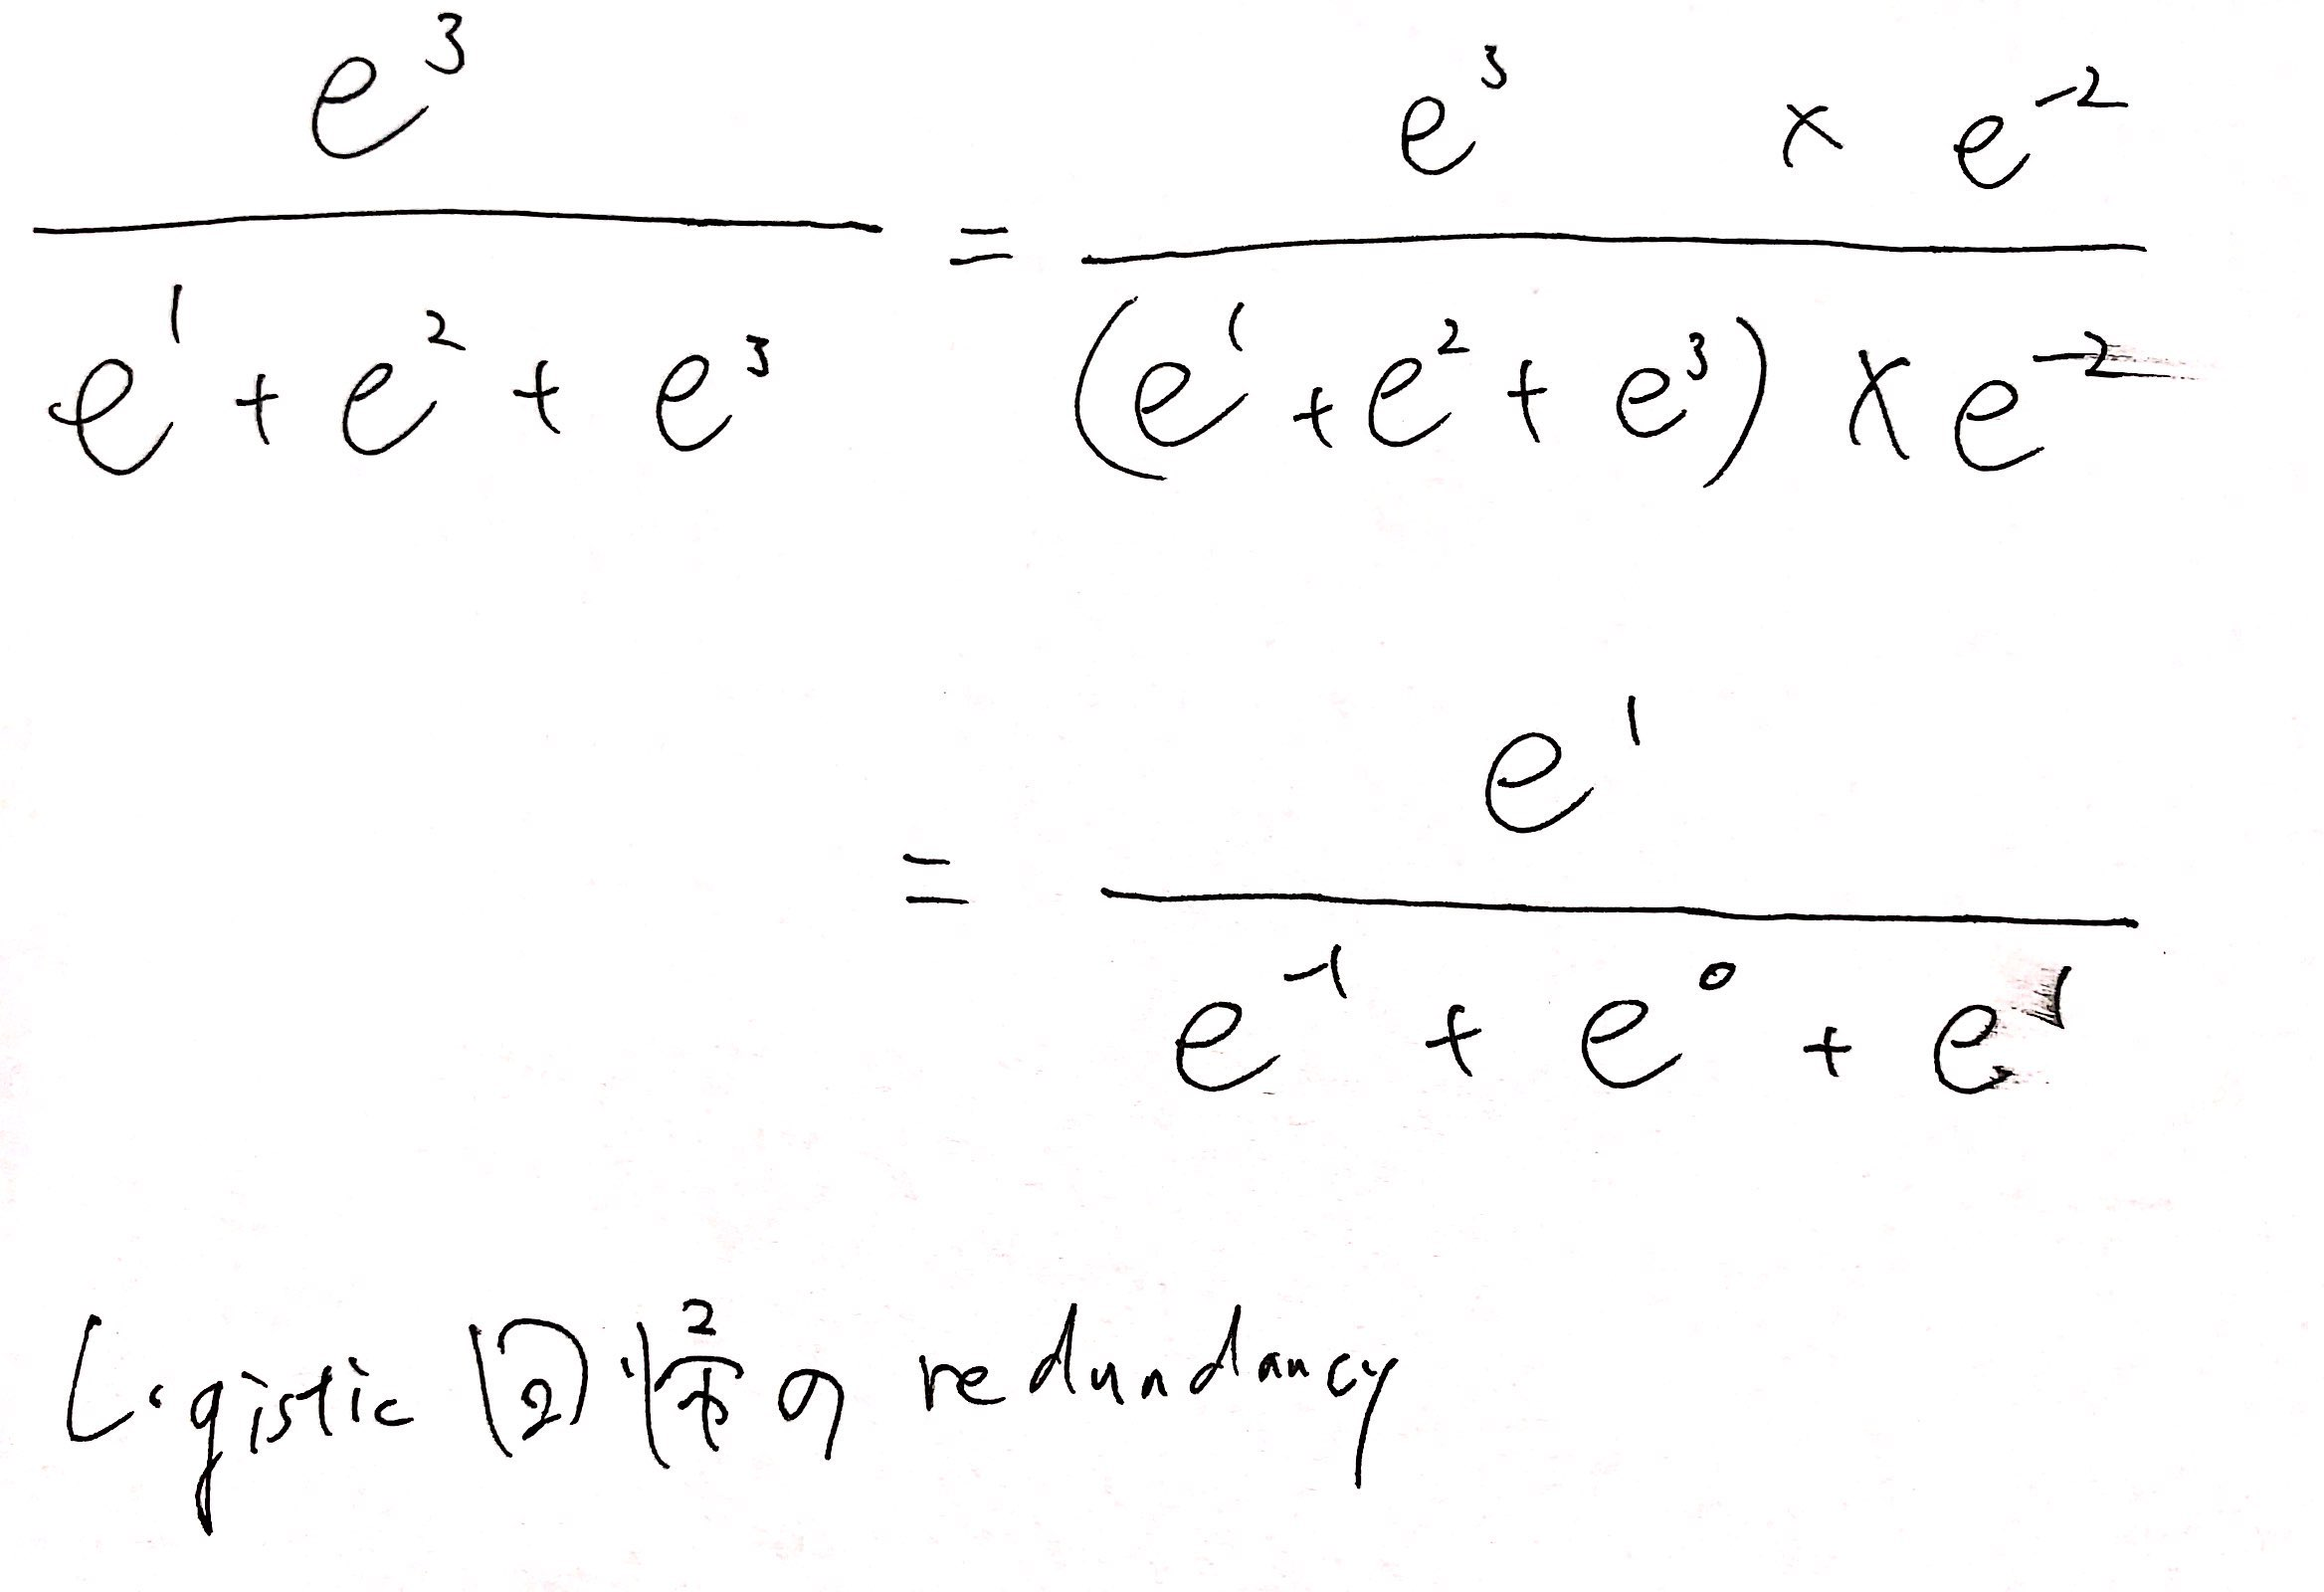
\includegraphics[width=4cm]{./images/logistic-redundancy.jpg}
    \end{figure}
  \end{frame}
  \begin{frame}{ロジスティック回帰}
    \begin{itemize}
      \item 前述の最大化問題は凸なので, Newton 法とかで解ける.
      \item separable なデータに対して, $\lambda\to 0$とすると, マージン最大化と同じ結果になる.(?) \\
        → SVM もうまく関連付けられそう.
    \end{itemize}
  \end{frame}
  \begin{frame}{Support Vector Classifier}
    \begin{itemize}
      \item 前に出てきた話. マージン最大化.
      \item $p \gg N$のとき, ほぼ確で線型分離可能なので, attractive.
      \item 正則化しなくても有効. 頑張って正則化しても, 正則化なしと同程度のパフォーマンスのことが多い.
      \item 多数のクラスへの分類への応用方法を2つ紹介.
        \begin{itemize}
          \item one versus one (ovo)\\
            全ての2つのクラスの組み合わせ($K(K-1)/2$通り)全てについて, SVMで分類する. \\
            点xについて, 上記の分類全ての結果, 最も多く分類されるクラスを推定値とする.
          \item one versus all (ova)\\
            各クラスとそのクラス以外に分けてSVMで分類する. \\
            教会からの符号付き距離(confidence)が最も大きいクラスを推定値とする.
        \end{itemize}
        ovo と ova は SVC に限らず使える手法.
      \item 正則化ロジスティック回帰と近しい結果を返す.
    \end{itemize}
  \end{frame}
  \begin{frame}{特徴量選択}
    \begin{itemize}
      \item $p$が大きい時, 特徴量選択は重要. 解釈可能性のため.
      \item DLDA, LR, SVC は, アルゴリズム内に特徴量選択の機能を含まない. (二次正則化のため)\\
        →外付けの特徴量選択手法が提案されている.
      \item 例. Recursive Feature Elimination.\\
        重みの小さい特徴量から無視していく. \\
        →あまり上手くいかないらしい. \\
        (`` we do not have an explanation for this behavior.'')
      \item Kernel 法使って外れ値に強くさせることも可能.
    \end{itemize}
  \end{frame}
  \begin{frame}{計算の工夫}
    $p \gg N$で二次正則化の線形モデルを考えた時に使える計算の工夫について. \\
    まずは最も簡単な ridge 回帰について.
    \begin{itemize}
      \item 以下の最小化を考える.
        \[
          \sum_{i=1}^N\left(y_i-\beta_0+\sum_{j=1}^px_{ij}\beta_j\right) ^2+\lambda\sum_{j=1}^p\beta_j^2
        \]
      \item これは, 解けて解は以下.
        \[
          \hat{\beta}=(\textbf{X}^\mathrm{T}\textbf{X}+\lambda\textbf{I})^{-1}\textbf{X}^\mathrm{T}\textbf{y}
        \]
      \item ここで, 行列$\textbf{X}$の特異値分解を考える.
        \[
          \textbf{X}=\textbf{U}\textbf{D}\textbf{V}^{\mathrm{T}}=\textbf{R}\textbf{V}^{\mathrm{T}}
        \]
      \item すると, 上記の解は以下になる.
        \[
          \hat{\beta}=\textbf{V}(\textbf{R}^\mathrm{T}\textbf{R}+\lambda\textbf{I})^{-1}\textbf{R}^\mathrm{T}\textbf{y}
        \]
      \item $\textbf{R}$を入力, $\textbf{y}$を出力としたときの ridge 回帰の結果を$\hat{\theta}$とすると, $\hat{\beta}=\textbf{V}\hat{\theta}$となっている.
      \item 結論, $p$次元データの回帰の計算を$N$次元データの計算に還元できる.
    \end{itemize}
  \end{frame}
  \begin{frame}{計算の工夫}
    ridge 回帰に関する考察は, より一般的な話につながる.
    \begin{itemize}
      \item 線形モデルを考える.
        \[
          Y=f(X)=\beta_0+X^{\mathrm{T}}\beta
        \]
      \item 任意の損失関数を取る.
        \[
          \sum_{i=1}^NL(y_i,f(x_i))
        \]
      \item 入力変数のデータの行列$\textbf{X}$を特異値分解して, $N\times N$行列$\textbf{R}$を作る.
        \[
          \textbf{X}=\textbf{U}\textbf{D}\textbf{V}^{\mathrm{T}}=\textbf{R}\textbf{V}^{\mathrm{T}}
        \]
      \item 以下の最小化を考える.
        \[
          (\hat{\beta}_0,\hat{\beta})=\mathrm{arg}\min_{\beta_0,\beta}\sum_{i=1}^NL(y_i,\beta_0+x_i^\mathrm{T}\beta)+\lambda\beta^\mathrm{T}\beta
        \]
        \[
          (\hat{\theta}_0,\hat{\theta})=\mathrm{arg}\min_{\theta_0,\theta}\sum_{i=1}^NL(y_i,\theta_0+r_i^\mathrm{T}\theta)+\lambda\theta^\mathrm{T}\theta
        \]
      \item すると, 以下が成り立つ.
        \[
          \hat{\beta}_0=\hat{\theta}_0,\hat{\beta}=\textbf{V}\hat{\theta}
        \]
    \end{itemize}
  \end{frame}
  \begin{frame}{計算の工夫}
    \begin{itemize}
      \item LR, LDA, SVM など広く応用可能.
      \item $L_1$正則化の時には使えないので注意.
      \item $\lambda$は交差検証とかで.
    \end{itemize}
  \end{frame}
  \section{$L_1$正則化線形分類\\p. 661-}
\begin{frame}{$L_1$正則化線形分類}
    ここまで$L_2$正則化. ここから$L_1$正則化. 嬉しいポイントは勝手に特徴量選択してくれること.
    \begin{itemize}
      \item 例えば, lasso 回帰. 以下を最小化.
        \[
          \sum_{i=1}^N\left(y_i-\beta_0+\sum_{j=1}^px_{ij}\beta_j\right) ^2+\lambda\sum_{j=1}^p|\beta_j|
        \]
      \item $L_1$正規化は勝手に特徴量選択をしてくれる.
        \begin{figure}[htb]
          \centering
          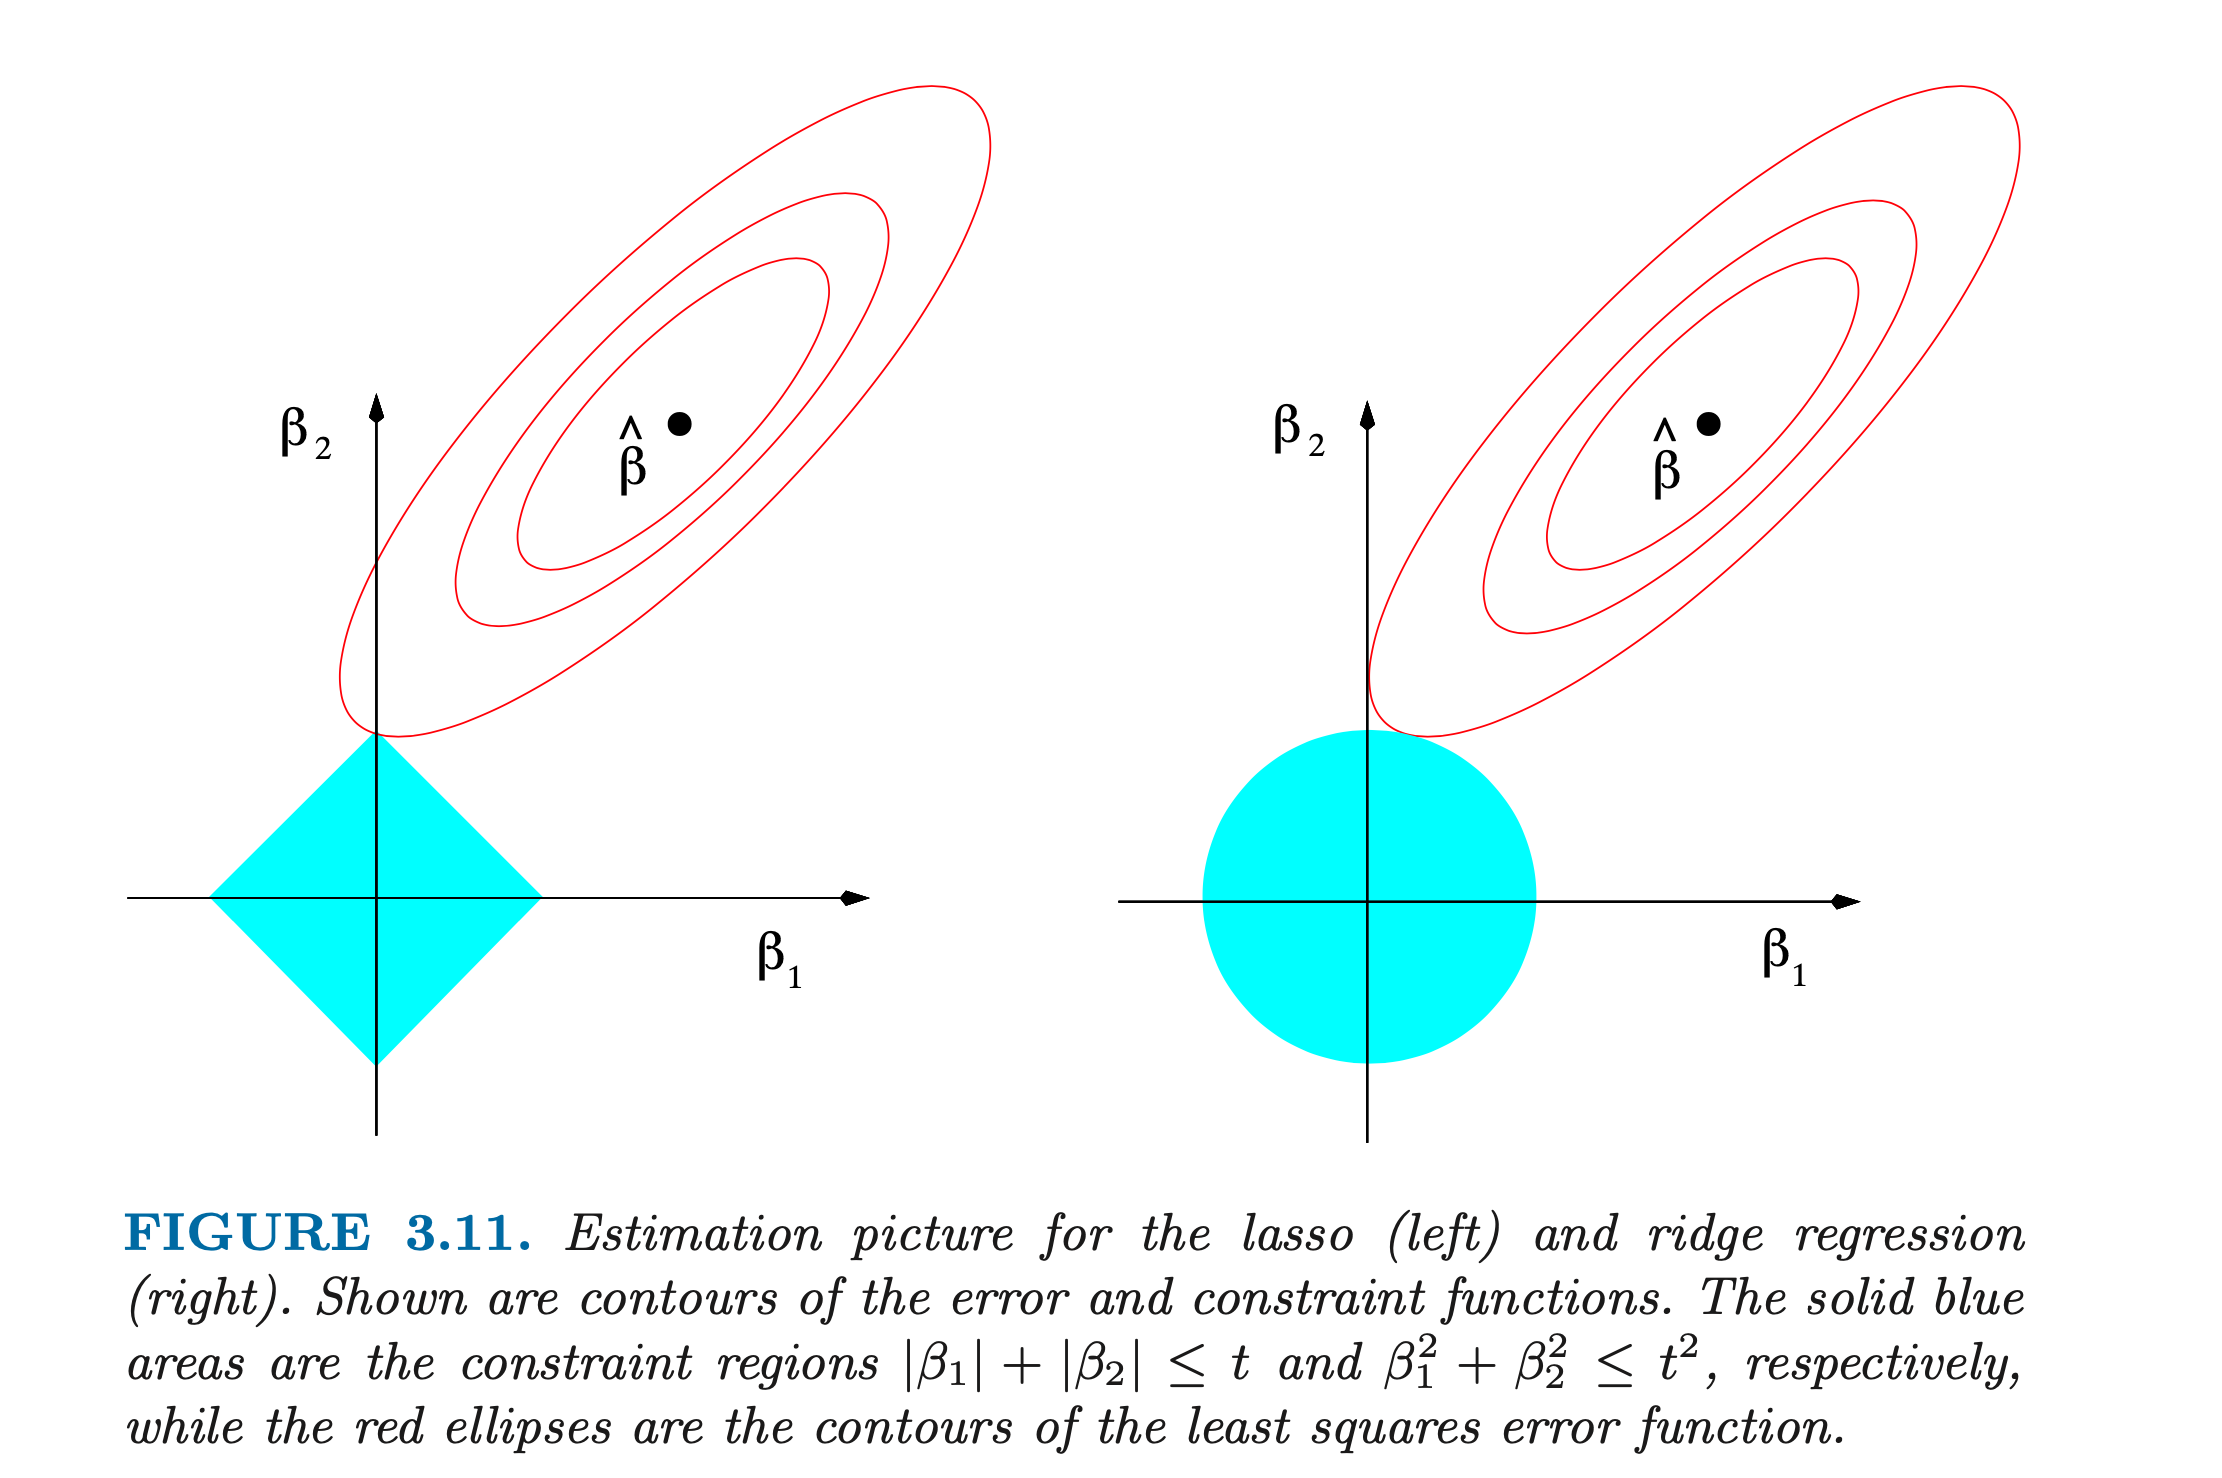
\includegraphics[width=5cm]{./images/automatic-feature-selection.jpg}
        \end{figure}
      \item 選ばれる特徴量は高々$N$個になる. (convex duality より. 凸共役?)
    \end{itemize}
  \end{frame}
  \begin{frame}{Elastic Net}
    \begin{itemize}
      \item $L_1$正規化の困るポイント. 相関の強い変数に対応できない. \\
        $Y=aX_1+b, X_2=X_1,a_1+a_2=a$とすると,
        \[
          Y=a_1X_1+a_2X_2+b
        \]
        となり, lassoでは$a_2,a_2$を特定できない.
      \item 回避策として, ridge と lasso の合体を考えるのが Elastic Net. 正則化項は以下.
        \[
          \sum_{j=1}^p(\alpha|\beta_j|+(1-\alpha)\beta_j^2)
        \]
      \item $alpha$は大抵 pre-chosen. もちろん, 交差検証でも良い.
    \end{itemize}
  \end{frame}
  \begin{frame}{Fused Lasso}
    特徴量たちが順序を持つ場合. 時系列データとか.
    \begin{itemize}
      \item 隣り合う特徴量について, 回帰係数を近づけたい. \\
        →以下を最小化する.
        \[
          \sum_{i=1}^N(y_i-\beta_0-\sum_{j=1}^px_ij\beta_j)^2+\lambda_1\sum_{j=1}^p|\beta|+\lambda_2\sum_{j=1}^{p-1}|\beta_{j+1}-\beta_j|
        \]
      \item 隣り合う特徴量の間隔が一定でないなら, それを考慮して以下を使う.
        \[
          \lambda_2\sum_{j=1}^{p-1}\frac{|\beta_{j+1}-\beta_j|}{|t_{j+1}-t_j|}
        \]
    \end{itemize}
  \end{frame}
  \begin{frame}{特徴量が明確でない場合 - String Kernel}
    分類したいけど, 特徴量がわからない場合. (タンパク質の構造)\\
    分類したいけど, あまりにも次元が大きすぎる場合. (文書の分類)

    →(非)類似度が測れればいろいろできる.

    \vspace{\baselineskip}

    タンパク質の構造による分類の例
    \begin{itemize}
      \item タンパク質は20種類のアミノ酸からなる列. 文字列で表せる.
        \begin{figure}
          \centering
          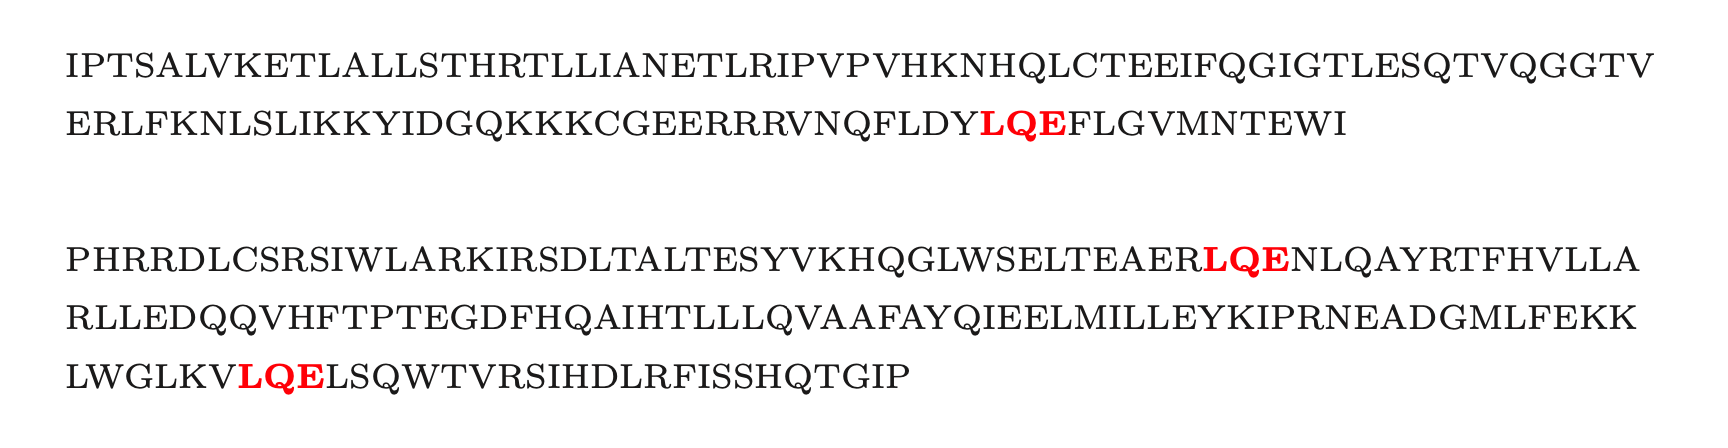
\includegraphics[width=5cm]{./images/protains.png}
        \end{figure}
      \item 部分文字列は良い特徴量になる. タンパク質$x$と$m$文字のアミノ酸列$a$に対して,
        $\varphi_a(x)$を$x$に含まれる$a$の数とする.
      \item 特徴量を
        \[
          \Phi_m(x)=\{\varphi_a(x)\}_{a\in\mathcal{A}_m}
        \]
        で定める.
      \item 類似度を内積として,
        \[
          K_m(x_1,x_2)=\langle\Phi_m(x_1),\Phi_m(x_2)\rangle
        \]
        で定める. (ちょっとRKHS感出てきた. )
      \item あとは, SVMとかすれば良い.
    \end{itemize}
  \end{frame}
  \begin{frame}{Kernelization}
    \begin{itemize}
      \item 様々な手法を``カーネル化''することができる. 簡単にいうと, データそのものの値ではなく, 各データの組の内積(類似度)や距離(非類似度)に注目しようという話. RKHS感が出てきている.
      \item 内積や距離の情報から計算できるモデルの例.\\
        SVM, 最近傍法, ロジスティック回帰, 主成分.
    \end{itemize}
  \end{frame}
  \begin{frame}{k-NN の Kernelization}
    内積の情報をもとにK近傍を見つけるために, 以下を用いれば良い.
    \[
      ||x_i-x_{i'}||^2=\langle x_i,x_i\rangle+\langle x_{i'},x_{i'}\rangle-2\langle x_i,x_{i'}\rangle
    \]
  \end{frame}
  \begin{frame}{Nearest Centroid の Kernelization}
    K-NN と似たイメージで,  Nearest Centroid 法もカーネル化できる.
    \[
      ||x-\bar{x}_k||^2=\langle x,x\rangle-\frac{2}{N_k}\sum_{g_i=k}\langle x,x_i\rangle+\frac{1}{N_k^2}\sum_{g_i=k}\sum_{g_j=k}\langle x_i,x_j\rangle
    \]
  \end{frame}
  \begin{frame}{ロジスティック回帰の Kernelization}
    \url{https://www.ism.ac.jp/~fukumizu/svm-ism.pdf}
    \begin{itemize}
      \item ロジスティック回帰の Lagrange Dual Form は以下.
        \[
          L_D=\sum_{i=1}^N\alpha_i-\frac{1}{2}\sum_{i=1}^N\sum_{i'=1}^N\alpha_i\alpha_{i'}y_iy_{i'}\langle x_i,x_{i'}\rangle
        \]
    \end{itemize}
  \end{frame}
  \begin{frame}{PCA の Kernelization}
    \begin{itemize}
      \item データ行列$\textbf{X}$の特異値分解を$\textbf{X}=\textbf{UDV}^{\mathrm{T}}$とすると, 主成分は以下.
        \[
          \textbf{Z}=\textbf{UD}
        \]
      \item ここから, 簡単に, 主成分をデータの分散共分散行列の対角化として得られることがわかる. (略)
      \item 分散共分散行列
        \[
          \hat{\textbf{K}}=(\langle x_i-\bar{x}, x_{i'}-\bar{x}\rangle)_{i,i'}
        \]
        なので, Kernelization できている.
    \end{itemize}
  \end{frame}
  \begin{frame}{Kernelization でできないこと}
    最適化を内積のみを用いて表すのは便利. じゃあできないことは?
    \begin{itemize}
      \item 変数の標準化
      \item 各変数の寄与の推定
      \item 効果のない変数と効果のある変数の見分け
    \end{itemize}
    総じて, 一つ一つの入力変数に注目は出来ない, というのが弱み.
  \end{frame}
  \section{余談 - 再生核ヒルベルト空間\\(Reproducing Kernel Hilbert Space, RKHS)}
  \begin{frame}{今こそRKHS - カーネル法(Kernel Method)}
    \begin{itemize}
      \item まずはカーネル法について, やりたいこととざっくり全体像の整理. \\
        \begin{itemize}
          \item 線形に分類できないもの(同心円が典型例)をうまく分類したい.
          \item 変数変換してあげると, 線形の手法を使える. \\
            \[
              (x,y) \mapsto (x^2,y^2)
            \]
          \item 高次元に写せば, ほぼ確実に線形分類可能にできる.
            \[
              (x,y)\mapsto (x,y,x^2,xy,y^2)
            \]
          \item 一方, 高次元に写すと計算量が増える. 困る. \\
            →高次元でも計算が楽なものはないのか...
          \item 数学の話. 再生核ヒルベルト空間(RKHS)という数学的対象とカーネル関数というある条件を満たす関数が1対1対応する.
            \begin{itemize}
              \item 再生核ヒルベルト空間は, 高次元に写す先の空間に相当. 
              \item カーネル関数は, 高次元空間における内積を直接計算する関数に相当. 
            \end{itemize}
          \item RKHSは内積計算が楽!内積で計算できるモデルならいい感じに使える!\\
            (SVM, CPA, etc...先述のものたちとか)
          \item 例えば, 以下を考える. 
            \[
              \Phi\colon \mathbb{R}^2\to\mathbb{R}^3, \Phi(x_1,x_2)=(x_1^2,x_2^2,\sqrt{2}x_1x_2)
            \]
            対応するRHKSは$\mathbb{R}^3$.
            カーネル関数は, 
            \begin{eqnarray*}
              K(x,y)&=&\langle(x_1^2,x_2^2,\sqrt{2}x_1x_2),(y_1^2,y_2^2,\sqrt{2}y_1y_2)\rangle\\
              &=&x_1^2y_1^2+x_2^2y_2^2+2x_1x_2y_1y_2\\
              &=&(x_1y_1+x_2y_2)^2\\
              &=&\langle x,y\rangle^2
            \end{eqnarray*}
        \end{itemize}
    \end{itemize}
  \end{frame}
  \section{Supervised Principal Component\\p. 674-}
  \begin{frame}{Supervised Principal Component}
    目的変数をよく説明できて, 分散が大きいような線形結合成分を取りたい. 
    \begin{figure}[htb]
      \centering
      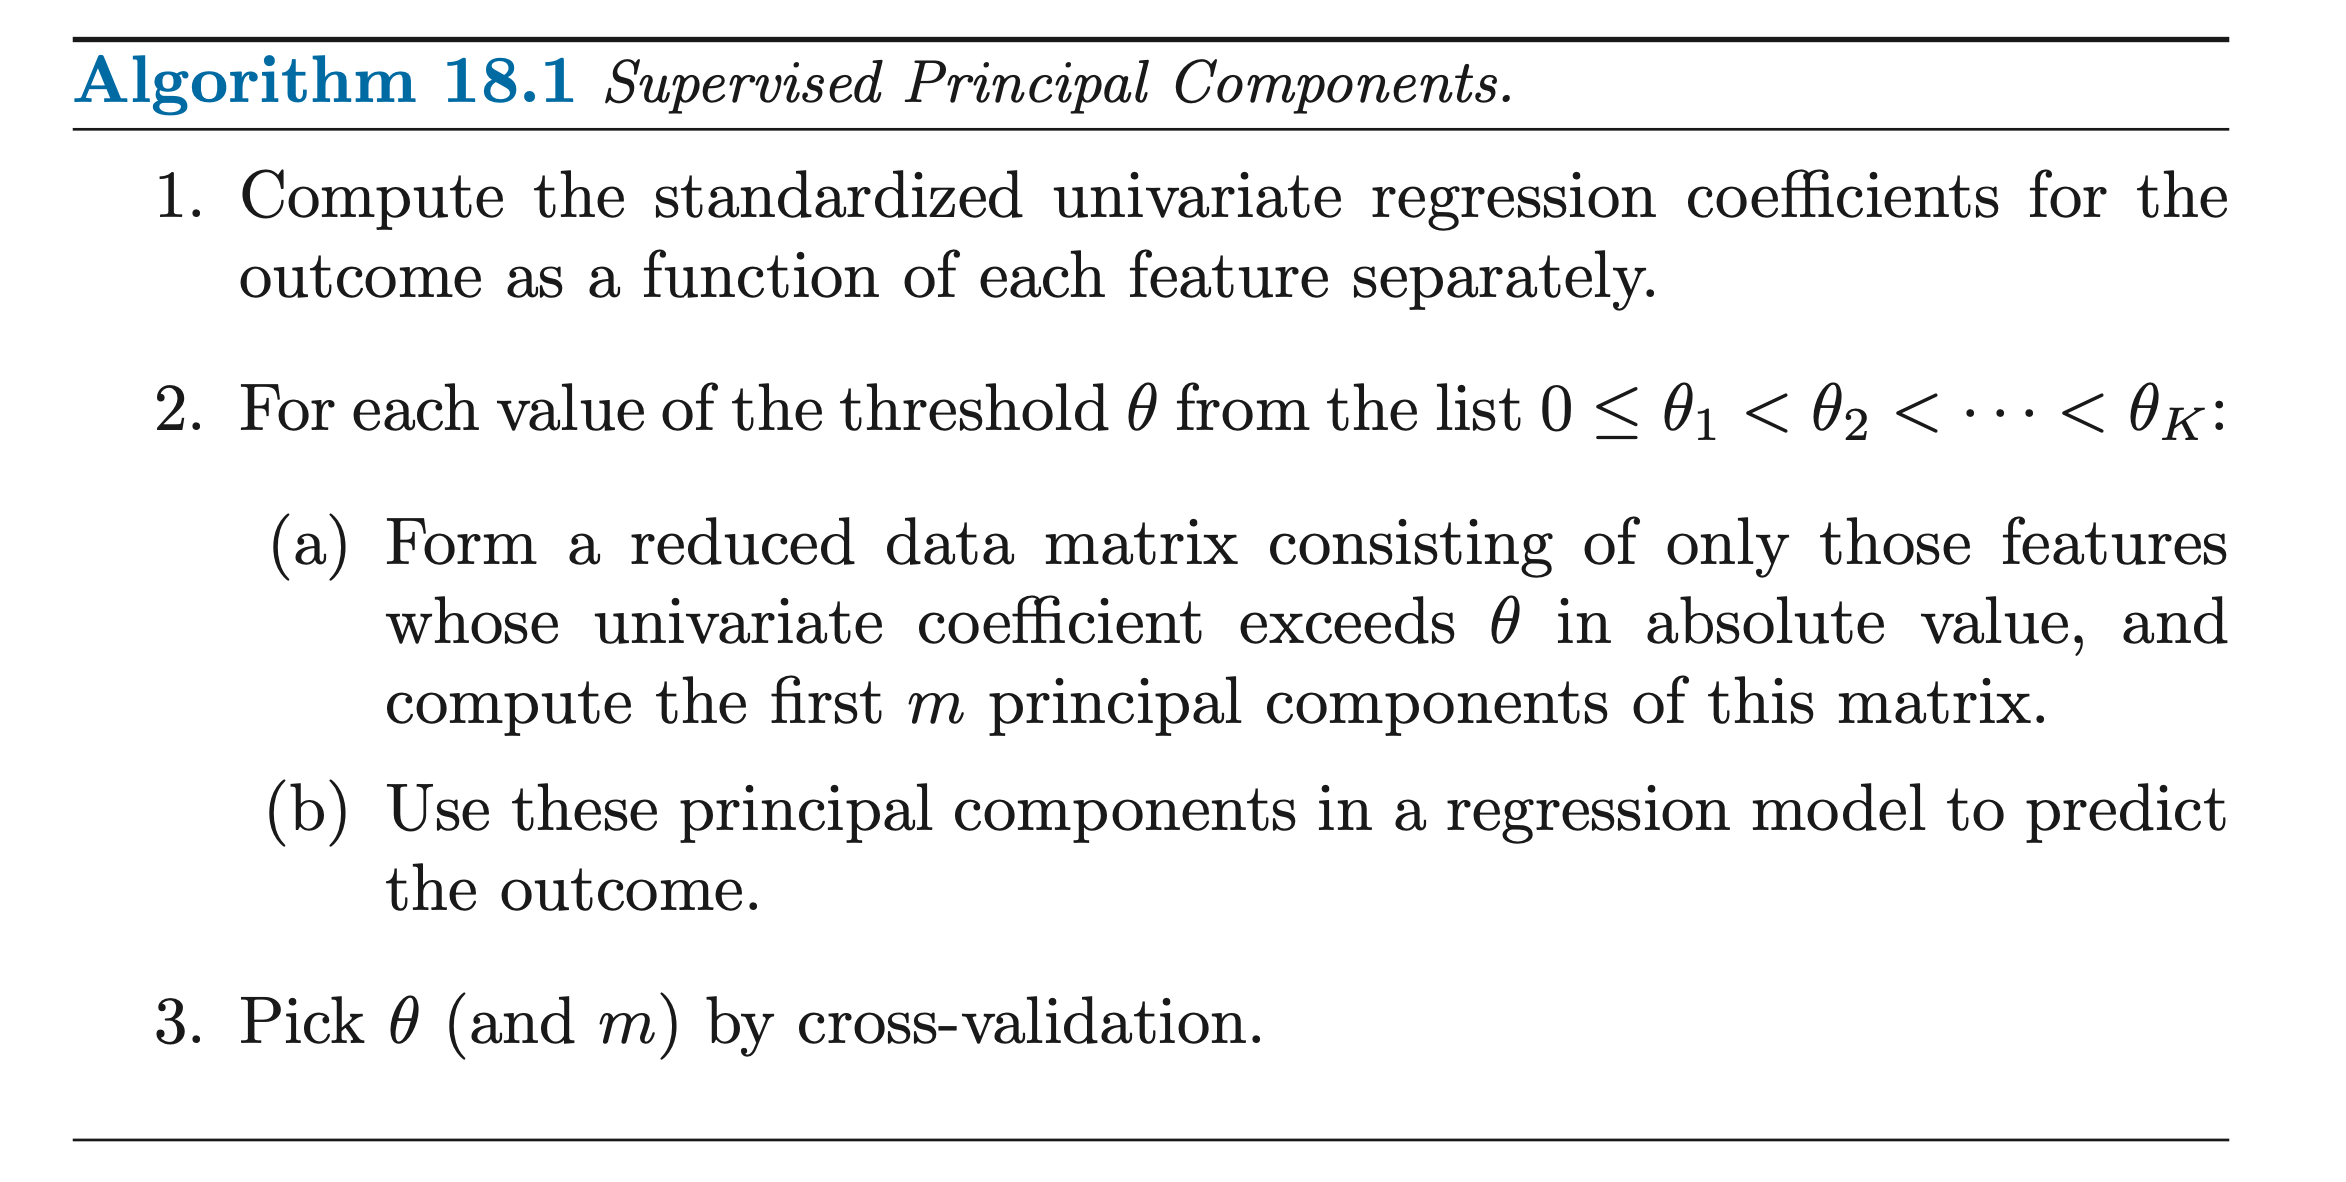
\includegraphics[width=8cm]{./images/supervised-pca.png}
    \end{figure}
    \begin{description}[Step. 2(a)]
      \item[Step. 1\ \ \ \ ] 普通に1変数線形回帰. 入力変数と目的変数の関係の強さを調べる.
      \item[Step. 2(a)] 変数選択からの主成分分析.
      \item[Step. 2(b)] 主変数での多変数回帰.
      \item[Step. 3\ \ \ \ ] 交差検証.
    \end{description}
  \end{frame}
  \begin{frame}{Supervised PCA と Partial Least Squares}
    3.5.2 で見た Partial Least Squares も, 説明力のある主成分を見つけようとする手法. 
    \begin{figure}[htb]
      \centering
      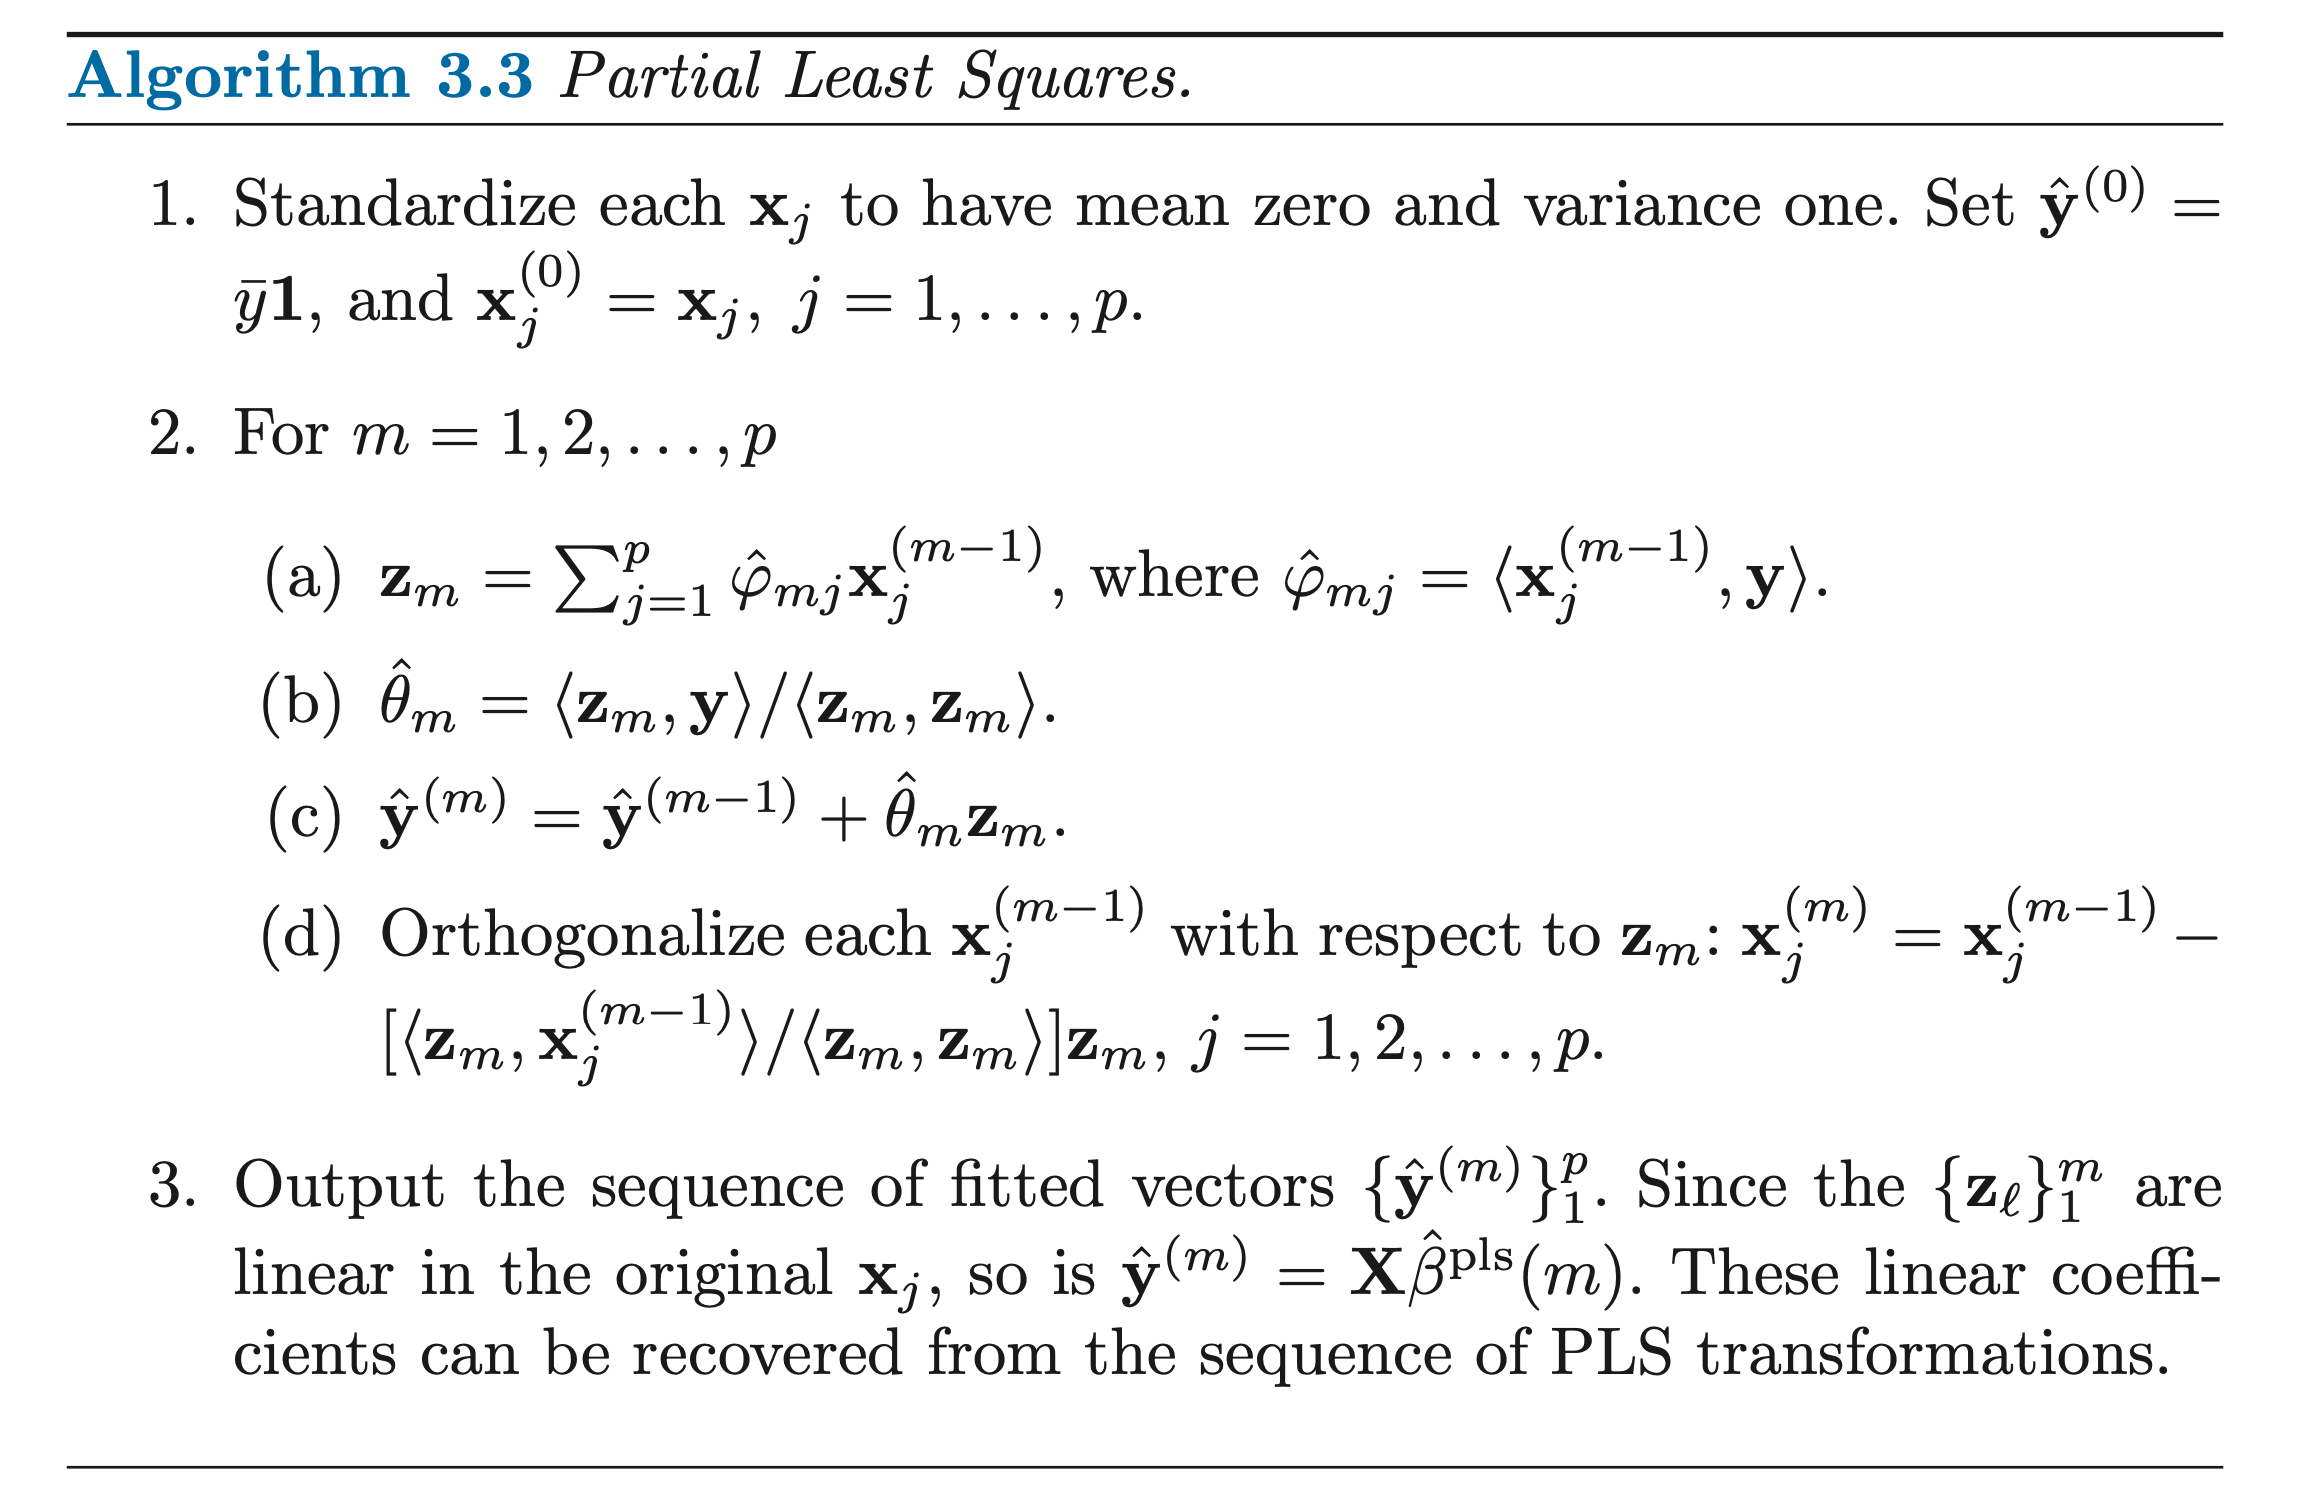
\includegraphics[width=8cm]{./images/pls.png}
    \end{figure}
    (アルゴリズム見てもイメージ湧かないかも)

    両者の違いは, SPCA は要らない特徴量を切り捨てるが, PLS は downweight するだけという点. 
  \end{frame}
\end{document}
